\documentclass[USenglish,glsresetperchapter,a4paper]{uit-thesis}

% Packages
\usepackage[utf8]{inputenc}
\usepackage{graphicx}
\usepackage{xspace}
\usepackage{tabularx}
\usepackage{amsmath}
\usepackage{numprint}
\usepackage{cases}
\usepackage{tocloft}
\usepackage{csquotes}
\usepackage{textgreek}
\usepackage{listings}
\usepackage[backend=biber, bibstyle=ieee, citestyle=numeric-comp, sorting=none]{biblatex}
\usepackage[binary-units=true]{siunitx}
\usepackage{subcaption}

% load configurations
\usepackage{tcolorbox}
\usepackage{xcolor}
\usepackage{varwidth}
\usepackage{environ}
\usepackage{xparse}

\newlength{\bubblesep}
\newlength{\bubblewidth}
\setlength{\bubblesep}{2pt}
\AtBeginDocument{\setlength{\bubblewidth}{.75\textwidth}}
\definecolor{bubblegreen}{RGB}{103,184,104}
\definecolor{bubblegray}{RGB}{241,240,240}

\newcommand{\bubble}[4]{%
  \tcbox[
    on line,
    arc=4.5mm,
    colback=#1,
    colframe=#1,
    #2,
  ]{\color{#3}\begin{varwidth}{\bubblewidth}#4\end{varwidth}}%
}

\ExplSyntaxOn
\seq_new:N \l__ooker_bubbles_seq
\tl_new:N \l__ooker_bubbles_first_tl
\tl_new:N \l__ooker_bubbles_last_tl

\NewEnviron{rightbubbles}
 {
  \begin{flushright}
  \sffamily
  \seq_set_split:NnV \l__ooker_bubbles_seq { \par } \BODY
  \int_compare:nTF { \seq_count:N \l__ooker_bubbles_seq < 2 }
   {
    \bubble{bubblegreen}{rounded~corners}{white}{\BODY}\par
   }
   {
    \seq_pop_left:NN \l__ooker_bubbles_seq \l__ooker_bubbles_first_tl
    \seq_pop_right:NN \l__ooker_bubbles_seq \l__ooker_bubbles_last_tl
    \bubble{bubblegreen}{sharp~corners=southeast}{white}{\l__ooker_bubbles_first_tl}
    \par\nointerlineskip
    \addvspace{\bubblesep}
    \seq_map_inline:Nn \l__ooker_bubbles_seq
     {
      \bubble{bubblegreen}{sharp~corners=east}{white}{##1}
      \par\nointerlineskip
      \addvspace{\bubblesep}
     }
    \bubble{bubblegreen}{sharp~corners=northeast}{white}{\l__ooker_bubbles_last_tl}
    \par
   }
   \end{flushright}
 }
\NewEnviron{leftbubbles}
 {
  \begin{flushleft}
  \sffamily
  \seq_set_split:NnV \l__ooker_bubbles_seq { \par } \BODY
  \int_compare:nTF { \seq_count:N \l__ooker_bubbles_seq < 2 }
   {
    \bubble{bubblegray}{rounded~corners}{black}{\BODY}\par
   }
   {
    \seq_pop_left:NN \l__ooker_bubbles_seq \l__ooker_bubbles_first_tl
    \seq_pop_right:NN \l__ooker_bubbles_seq \l__ooker_bubbles_last_tl
    \bubble{bubblegray}{sharp~corners=southwest}{black}{\l__ooker_bubbles_first_tl}
    \par\nointerlineskip
    \addvspace{\bubblesep}
    \seq_map_inline:Nn \l__ooker_bubbles_seq
     {
      \bubble{bubblegray}{sharp~corners=west}{black}{##1}
      \par\nointerlineskip
      \addvspace{\bubblesep}
     }
    \bubble{bubblegray}{sharp~corners=northwest}{black}{\l__ooker_bubbles_last_tl}\par
   }
  \end{flushleft}
 }
\ExplSyntaxOff
% Code listings
\definecolor{deepblue}{rgb}{0,0,0.5}
\definecolor{deepred}{rgb}{0.6,0,0}
\definecolor{deepgreen}{rgb}{0,0.5,0}
\colorlet{punct}{red!60!black}
\definecolor{background}{HTML}{EEEEEE}
\definecolor{delim}{RGB}{20,105,176}
\colorlet{numb}{magenta!60!black}

\DeclareFixedFont{\ttb}{T1}{txtt}{bx}{n}{12} % for bold
\DeclareFixedFont{\ttm}{T1}{txtt}{m}{n}{12}  % for normal
\lstset{
    language=python,
    basicstyle=\ttm,
    otherkeywords={self},             % Add keywords here
    keywordstyle=\ttb\color{deepblue},
    emph={Slave,__init__, start, header, row, stop},          % Custom highlighting
    emphstyle=\ttb\color{deepred},    % Custom highlighting style
    stringstyle=\color{deepgreen},
    frame=tb,                         % Any extra options here
    showstringspaces=false            % 
}

\lstdefinelanguage{json}{
    basicstyle=\ttm,
    numberstyle=\scriptsize,
    stepnumber=1,
    numbersep=8pt,
    showstringspaces=false,
    breaklines=true,
    literate=
     *{0}{{{\color{numb}0}}}{1}
      {1}{{{\color{numb}1}}}{1}
      {2}{{{\color{numb}2}}}{1}
      {3}{{{\color{numb}3}}}{1}
      {4}{{{\color{numb}4}}}{1}
      {5}{{{\color{numb}5}}}{1}
      {6}{{{\color{numb}6}}}{1}
      {7}{{{\color{numb}7}}}{1}
      {8}{{{\color{numb}8}}}{1}
      {9}{{{\color{numb}9}}}{1}
      {:}{{{\color{punct}{:}}}}{1}
      {,}{{{\color{punct}{,}}}}{1}
      {\{}{{{\color{delim}{\{}}}}{1}
      {\}}{{{\color{delim}{\}}}}}{1}
      {[}{{{\color{delim}{[}}}}{1}
      {]}{{{\color{delim}{]}}}}{1},
}

\renamedefname{lstlistlisting}{List of Code Listings}
\renamedefname{lstlisting}{Code Listing}
\renameautorefname{lstlisting}{code listing}
\urlstyle{rm}
\newglossarystyle{ult-super}{
    \setglossarystyle{ult-long}
    \setlength{\glsdescwidth}{0.74\textwidth}
    \renewcommand*{\glossentry}[2]{
        \glsentryitem{##1}\glstarget{##1}{\glossentryname{##1}} &
        \glossentrydesc{##1}\glspostdescription\space ##2\tabularnewline&\tabularnewline%
    }
}
\makenoidxglossaries
\loadglsentries{acronyms}
\newcolumntype{R}{>{\raggedleft\arraybackslash}X}
\newcommand{\tab}{\hspace*{10em}}
% List of equations
\newcommand{\listequationsname}{List of Equations}
\newlistof{myequations}{equ}{\listequationsname}
\newcommand{\myequations}[1]{%
\addcontentsline{equ}{myequations}{\protect\numberline{\theequation}#1}\par}

% Paths
\addbibresource{bibliography.bib}
\graphicspath{{images/}}

% Thesis configuration
\ThesisRightFrontpageImage{images/longcat_flip.jpg}
\newcommand{\project}{Limelight\xspace}
\newcommand{\thesisquote}[2]{\emph{“#1”} -- #2 \\[2\baselineskip]}

\begin{document}
% Front page
\title{\project: Real-Time Detection of Pump-and-Dump Events on Cryptocurrency Exchanges Using Deep Learning}
\author{Andreas Isnes Nilsen}
\thesisfaculty{The Faculty of Science and Technology \\ Department of Computer Science}
\thesisprogramme{INF-3981: Master's Thesis In Computer Science \\ June 1st 2019}
\maketitle
\frontmatter

% Meta
\begin{center}
    
\includegraphics[width=\textwidth]{images/longcat.jpg}
\end{center}
\vspace*{\fill}

\begin{flushright}
    \thesisquote{Long cat, is long.}{Robert Pettersen}
    \thesisquote{Fått laksekrem på hjernen.}{Maren Sofie Ringsby}
    \thesisquote{Reality continues to ruin my life.}{Bill Watterson}
\end{flushright}
% Abstract: each about 1/2 page
% http://williamstallings.com/Extras/Abstract.html
% Motivation (Why do we care?)
% Problem statement (What problem are we trying to solve?)
% Approach (How did we go about it)
% Results (What’s the answer?)
% Conclusion (What are the implications of the answer?)

\begin{abstract}
% Glory
Following the birth of cryptocurrencies back in 2008, virtual investment platforms called exchanges were created to integrate these cryptocurrencies into their platform. Allowing investors to sell and buy assets fairly and agile. Exchanges now, has become so popular and carry out over $99\%$ of all the transactions, and every day over hundreds of million dollars in worth of cryptocurrencies are traded 


% Dark

% Solution

\end{abstract}
\begin{acknowledgement}
Bjørn Hellfuck er fette gudis
\end{acknowledgement}
\tableofcontents
\listoflistings
\listofmyequations
\printacronyms[style=ult-super]

% Content
\mainmatter

\chapter{Introduction}\label{ch:introduction}

\section{Problem Definition}\label{sec:problem_definition}

\section{Context}\label{sec:context}
This thesis is written in the context of Corpore Sano Centre\footnote{http://www.corporesano.no/}, a center for sport and health technology.


\newpage\section{Methodology}\label{sec:methodology}
The final report of the Task Force on the Core of Computer Science\cite{computing_as_a_discipline} define the succeeding three major paradigms as the discipline of computing.

The first paradigm, \emph{theory}, is rooted in mathematics and consists of four steps followed in the development of a coherent, valid theory: 
\begin{enumerate}
    \item characterize objects of study (definition);
    \item hypothesize possible relationships among them (theorem);
    \item determine whether the relationships are true (proof); 
    \item interpret results.
\end{enumerate}

The second paradigm, \emph{abstraction} (modeling), is rooted in the experimental scientific method and consists of four stages that are followed in the investigation of a phenomenon: 
\begin{enumerate}
    \item form a hypothesis;
    \item construct a model and make a prediction;
    \item design an experiment and collect data;
    \item analyze results.
\end{enumerate}

The third paradigm, \emph{design}, is rooted in engineering and consists of four steps followed in the construction of a system (or device) to solve a given problem:
\begin{enumerate}
    \item state requirements; 
    \item state specifications;
    \item design and implement the system;
    \item test the system.
\end{enumerate}

\section{Outline}\label{sec:outline}
\begin{itemize}
    \item[] \textbf{\autoref{ch:background}}
    \item[] \textbf{\autoref{ch:design}}
    \item[] \textbf{\autoref{ch:implementation}}
\end{itemize}
% Fundamentals / environment and related work: 1/3
% comment on employed hardware and software
% describe methods and techniques that build the basis of your work
% review related work(!)

\chapter{Background and Related Work}\label{ch:background}\glsresetall
\section{Cryptocurrency}\label{sec:cryptocurrencies}
% What is cryptocurrency???
Cryptocurrencies are digital or virtual assets, and they use cryptography as a security and consistency mechanism~\cite{investopedia_cryptocurrency, P&D_to_the_moon}. The majority of cryptocurrencies are decentralized systems built on \emph{blockchain} technology, a public tamper proof transaction ledger. With the blockchain, any arbitrary person can verify the consistency of transactions without linking them to real-world identities. Satoshi Nakamoto is the founder of the first and most prevailing cryptocurrency from 2009, namely Bitcoin. In recent years, the number of other cryptocurrencies called \emph{altcoins} have emerged, and at the time writing, there are now over $2000$ different cryptocurrencies~\cite{coinmarketcap}. The altcoins describe themselves as better substitutes as Bitcoin face various complications which \autoref{sec:blockchain} details. Besides Bitcoin, other popular cryptocurrencies are Ripple, Ethereum, XRP, and Litecoin.

% Incentive
Traditional payment systems suffer from the inherent weakness of the trust based model. Completely non-reversible 
transactions are not possible since financial institutions cannot avoid mediating disputes. With the possibility of reversal, the need for trust spreads making merchants prompt customers for their confidential~\cite{bitcoin}. In contrast, cryptocurrency transactions are irreversible, Bitcoin defines an electronic payment as a chain of digital signatures, each transfer are digitally signed with the previous transaction~\cite{bitcoin, ethereum_white}. Cryptocurrency systems are pseudonymous; the public sees all the transactions, but without linking them to real-world identities.

\begin{figure}[ht]
    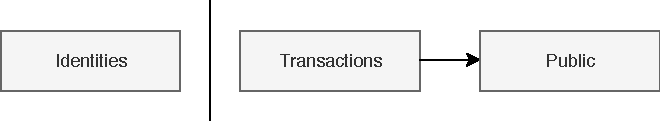
\includegraphics[width=\textwidth]{cryptocurrency_model.pdf}
    \caption{Privacy model for Bitcoin and the majority of altcoins (Source: \cite{bitcoin}).}
    \label{fig:cryptocurrency_model}
\end{figure}

% Issues
Problems originate with the privacy model of Bitcoin and the majority of altcoins, see \autoref{fig:cryptocurrency_model}. According to \cite{bitcoin_regulation}, the emergence of cryptocurrencies has raised significant concerns about potential illegal activities, such as terrorism and money laundering, customer theft and fraud. The expansion of cryptocurrencies may also threaten the traditional money issuance system, question the role of banks and other financial institutions in funds transfers and present a risk for the financial stability in general.

\subsection{Blockchain}\label{sec:blockchain}
% What is a blockchain???
A blockchain~\cite{bitcoin_book} is an ever growing list of blocks, equivalent to a list \ac{adt}~\cite{bitcoin_book}. Blocks in a blockchain consists of data and a \emph{hash pointer}, a reference to and a cryptographic hash of the previous block, see \autoref{fig:blockchain}. Whereas a regular pointer makes it possible to retrieve a blocks location in memory, a hash pointer also makes it possible to verify the integrity of the data. With other words, it is possible to check if the data within a block have changed after the creation of it. In the context of cryptocurrency, blocks contain metadata and a series of transactions.

\begin{figure}[ht]
    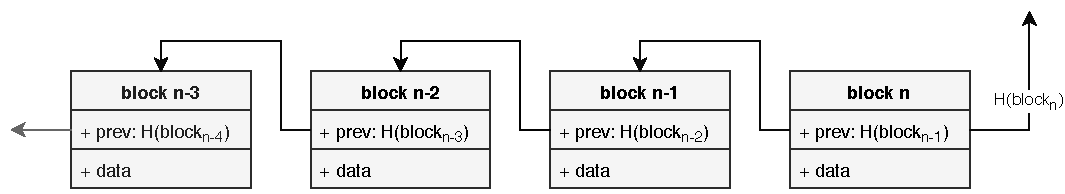
\includegraphics[width=\textwidth]{blockchain.pdf}
    \caption{Abstract view of a blockchain}
    \label{fig:blockchain}
\end{figure}

% Miners and PoW
For nodes (miners) in cryptocurrency systems to solve the double-spending problem and agree on the succeeding block of pending transactions, they all must agree on a single block that comes next in line in the blockchain. The majority of cryptocurrencies use the consensus protocol \ac{pow} to elect the next block, which we define as follows: Miners collect broadcasted pending transactions into a block; they are fussy and exclusively pick the transactions with the highest fees~\cite{trends_fee, trans_fee}. Then, the miners must play a cryptographic puzzle. They start hashing the new block with the hash of the previous block until the digest is below a defined threshold. Each try is pseudo-stochastic, so it requires indefinite attempts, and miners can flip a bit in the block-field \emph{nonce}, so they do not reuse the same digest. The first miner to solve the puzzle gets a minting reward and has to sign the blocks and broadcast it to the other miners which add the new block into the blockchain. Statistically, systems that use \ac{pow} remain their integrity as long as honest nodes possess more than $50\%$ of the total hashing rate in the system.
% Possibly add some inline definitions and functions for properly formalize it.
% NEED TO FIX: 
%   Each try is pseudostochastic so it... 


% Propegation time
The Bitcoin protocol defines the issuing rate of new blocks to be approximately ten minutes. After the immense interest in cryptocurrency, the amount of miner has skyrocket which results in high electricity expenditure and longer verification time of transactions due to the slower propagation time of blocks. Bitcoin miners electrical consumption alone can power five million U.S households and the emission of CO$_2$ for producing the required electricity is $275$ kilogram per transaction~\cite{bitcoin_power}. As the number of miners escalates, the longer propagation time of blocks, thus, the time-gap of where two or more block being proposed and integrated by miners at the same time expand~\cite{trans_fee}. When the miners have a different vision of the blockchain, they have created a \emph{branch}. Any branch is fixable though producing the longest branch as the \ac{pow} protocol looks at the longest branch as the true main branch. The blocks that are mined but was cut off from the main branch are invalid and called \emph{orphaned block}. And because of the possibility of orphaning, a rule of thumb in verification of Bitcoin transactions is to wait until a block with your payment is confirmed (buried under other blocks) six times~\cite{bitcoin_verification_1, bitcoin_verification_2} which is around one hour.

\subsection{Exchanges}\label{sec:exchanges}
% what are exchanges?
Cryptocurrency exchanges are centralized online platforms where traders can exchange cryptocurrency for another cryptocurrency or fiat\footnote{Money made by the government\cite{fiat}}. They are typically market makers that take \emph{bid-ask} spreads as transaction commissions for their services or charge fees as a matching platform~\cite{norton_rose}. Currently, they lack regulation\footnote{Application of law by the government} which makes them not trustworthy and susceptible to price manipulation schemes and con artists~\cite{exchange_scammers, exchange_scammers_2}. There are over $200$ different cryptocurrency exchanges where some of the most appealing are Coinbase, Binance, Bittrex, and Poloniex~\cite{exchange_best_1, exchange_best_2}, where Binance has a monthly trading volume of more than \$$20$ billion~\cite{coinmarketcap_exchange}.

% trading pairs
Cryptocurrency exchanges list various symbol pairs denoting a \emph{base} and \emph{quote}. The currency pairs compare the value of one currency to another - the base currency versus the quote. It indicates how much of the quote currency is needed to purchase one unit of the base currency~\cite{investopedia_cryptocurrency}. Furthermore, exchanges categorize symbol pairs in markets, where the quote are typically the name of the market. For example, to trade Ethereum (ETH) for Bitcoin (BTC), the symbol pair "ETH/BTC" is in the Bitcoin market along with countless other symbol pairs.

% tokens
Trades on cryptocurrency exchanges are with \emph{tokens} which makes them off-blockchain~\cite{exchange_off_chain}, but in return, there is no need for verification as trades happening instantly. However, traders seemingly prefer to use multiple exchanges simultaneously, and transaction between exchanges are registered on the cryptocurrency's blockchain, see \autoref{fig:exchanges}. Exchanges are contradictory to the incentive of cryptocurrencies as they are decentralized systems while exchanges are centralized, but still, $99\%$ of cryptocurrency trades happen on exchanges~\cite{coinsutra}.
%% NEED TO REWRITE

\begin{figure}[ht]
    \centering
    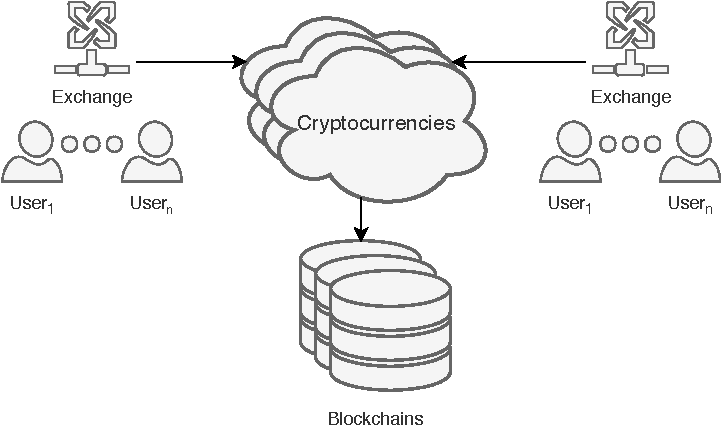
\includegraphics[width=\textwidth]{exchanges.pdf}
    \caption{Cryptocurrency exchanges ecosystem}
\label{fig:exchanges}
\end{figure}

\subsubsection{Market data}
% rest api
Before the internet, trading, in general, took place over the phone, in the post-internet age, trading takes effect over an exchange's \ac{api}~\cite{exchange_api} allowing software to pull data and interact with the exchange. \acp{api} are useful analytics and for traders who have algorithmic models that are fueled by live data and need to issue orders within milliseconds.

\subsubsection{OHLCV}
Graphical illustrations of price movements for specific time intervals goes by the name \emph{kline} or \emph{candlestick} chart. Such graphs utilize a set of \acp{ohlcv} points, describing the trading trends in a time window. \autoref{tab:ohlcv} illustrates a candle in its crude form, and \autoref{fig:pd-gxsbtc} shows processed \acp{ohlcv} values making a candlestick chart. The top and bottom wicks represent the highest and lowest trade price respectively in the time interval, while the color portrays whether the closing price was higher or lower than the opening price~\cite{P&D_to_the_moon}. Candles can define trading trends in any time interval, but exchange’s \ac{api} mostly allows a discrete selection of timeframes that commonly range from one minute to several days.
\begin{table}[ht]
    \centering
    \begin{tabular}{ c c c c c c }
        \hline
        \textbf{Timestamp} & \textbf{Price} & & & & \textbf{Trading volume} \\
        \cline{2-5}\\
                  & \textbf{Open}  & \textbf{High} & \textbf{Low} & \textbf{Close} & \\
        \hline
        2019-06-01 23:59:59 & $2006.2$ &  $2061.3$ & $1926.2$ & $1984.1$ & $216304.7$\\
        \hline
    \end{tabular}
    \caption[Structure - \Acf{ohlcv}]{shows the structure of an \acp{ohlcv} value. The volume presents the number of assets that were traded over a period. The price field denotes the highest and lowest price that was recorded, as well as the price from where the period started (open) to where it ended (close).}
    \label{tab:ohlcv}
\end{table}



\subsubsection{Order Book}
% Order book
% Level 1 & Level 2
An order book also aliased market depth is an electronic list of buying and sell orders on an exchange for a specific symbol pair, see \autoref{tab:order_book}~\cite{investopedia_depth}. Sell orders are in an \emph{asks} list in a descending order while buy orders are arranged descendingly in a \emph{bids} list~\cite{invest_order_book, coincodex_order_book}. The order book is dynamic and constantly change throughout the day as traders are issuing new orders. There are many ways to interpret an order book; for instance, a massive imbalance of buy orders versus sell orders may indicate a price increase due to buying pressure~\cite{invest_order_book}.
\begin{table}[ht]
    \centering
    \begin{tabular}{c c| c c}
        \hline
         \textbf{Asks} & & \textbf{Bids} & \\
         \textbf{Price} & \textbf{Volume} & \textbf{Price} & \textbf{Volume}\\
         \hline
         [$0.028$ ... $0.14$] & [$12.4$ ... $3.1$] & [$0.027$ ... $0.018$] & [$56.4$ ... $1.45$]\\
         \hline
    \end{tabular}
    \caption[Structure - Order book]{shows the structure of an order book. The left side (askers) includes the quantity of coins that are buyable, while the right side (bidders) are bids that are waiting to be matched against buyable coins. }
    \label{tab:order_book}
\end{table}

\subsection{Pump-and-Dump}\label{sec:pd}
A \ac{pd} scheme is a type of fraud in which the offenders accumulate a commodity over a period, then artificially inflate the price through means of spreading misinformation (pumping), before selling off what they bought to unsuspecting buyers at the higher price (dumping)\cite{P&D_to_the_moon}. After the emergence of cryptocurrency trading, \ac{pd} has become a popular legitimate price manipulation scheme among scammers, who leach assets from the misinformed. Two researchers at the Imperial College London revealed that on average, at least two \ac{pd} schemes are carried out daily, producing \$$7$ million in daily trading volume~\cite{P&D_MIT_crypto}. Price increases of up to 950\% have been witnessed, demonstrating the amount of potential profit~\cite{P&D_cointelegraph}.

% stock market
On the modern stock market, \ac{pd} schemes are internet-based focusing on \emph{penny} or \emph{microcap} stocks, which are smaller companies that do not comply with the standards to being listed on the larger exchanges~\cite{stock_bouraoui, stock_temple, P&D_anatomy}. Microcap stock exchanges are not held to the same standard of regulation, which implies that there are usually not as much information about the companies that are listed making them easier to manipulate~\cite{P&D_to_the_moon}. Misinformation about the stocks are usually spread through email spam which have a net positive effect on the stock price~\cite{stock_bouraoui}. It is illegal to run price manipulation schemes on regulated markets, and there are multiple cases where participants in a \ac{pd} are prosecuted~\cite{P&D_to_the_moon}.

% cryptocurrency market
There is a slightly different approach of \acp{pd} on the cryptocurrency market. The pump is a coordinated, intentional, short-term increase in the demand of a symbol pair~\cite{P&D_anatomy} organized by dedicated groups. These groups are often public channels in chat applications like Discord or Telegram and are joined by naive traders, who believe they will become wealthy in a short amount of time. The number of members in some of the prominent groups have peaked at circa $200,000$~\cite{P&D_the_outline}.

\subsubsection{Pump Groups}\label{sec:pump_groups}
% Group setup
In the cryptocurrency market, \ac{pd} organizers (admins) create groups in encrypted chatting application such as Telegram and Discord. They advertise themselves through social media platforms and forums~\cite{P&D_anatomy, P&D_scheme} as exciting groups that ensures profit with little or no risk of losing assets. The group admins start to organize \ac{pd} when the group typically consists of over $1,0000$ optimistic traders~\cite{P&D_anatomy}. Only the admins are allowed to post messages in the group restricting regular members to just see the messages posted by the admins; this functionality is enabled by the admins to avoid member interference~\cite{P&D_anatomy}.

% Accumulate
Before a \ac{pd}, the group admins announce details regarding it a few days ahead. The information they provide is the exact time and date, the quote which is more or less always Bitcoin, and the exchange. With the information, the member can buy sufficient funds on the targeted exchange in advance~\cite{P&D_anatomy}. The same day the \ac{pd} is scheduled, the admins purchase a commodity in the base coin over a period without raising the price. And they send out countdowns and reminds the members of previous successfully \acp{pd} to motivate them to participate, and the "rules" during the upcoming \ac{pd}. According to \cite{P&D_anatomy}, the typical rules are.

\begin{enumerate}
    \item Make sure to buy fast.
    \item \emph{Shill}\footnote{Cryptocurrency jargon for "promote" or "advertise" coin.} the announced coin on social media to attract outsiders.
    \item \emph{HODL}\footnote{Cryptocurrency jargon for Hold.} the coin for several minutes to give outsiders the possibility of joining.
    \item Sell in pieces at profit, not in chunks.
\end{enumerate}

% pump-and-dump
When the admins announce the coin, each member tries to be the first to buy the published coin to ensure profit before the inevitable inflation. If they are to slow, they might buy at the peak and are unable to make a profit. The pressure of being the first is high because the coin peak within seconds to max ten minutes~\cite{P&D_the_outline, P&D_anatomy}. After they have bought a significant amount of the coin, they shill, in an attempt to trick outsiders into buying it, allowing them to sell easier~\cite{P&D_anatomy}. The misinformation varies, but some common tactics include false news stories, non-existent projects, fake partnerships, or fake celebrity endorsements~\cite{P&D_the_outline}. Simultaneously, the admins encourage the members to hold while they sell off what they bought earlier on that day making them maximize their profit before the inevitable price dump. As soon as the first fall in price appears, the members start to panic-sell. If the price dips below the start price, the second wave of traders buys to bounce the price up to where it began allowing them to gain a small profit~\cite{P&D_anatomy}.

% post pump
Minutes to hours later, when the coin recover to its initial state. The admins publish results that showcases the members impact and the potential profit. \autoref{fig:chat_pump} shows real messages from \ac{pd} organized by the pump group Crypto Pump Island, and the \autoref{fig:pd-gxsbtc} shows the impact.

Nevertheless, in the end, only the admins and a few members are profiting from a \ac{pd} while the majority are loosing. So why are there still people enthusiastic about partaking a \ac{pd}, given the risk of being ripped off by the admins? Because people believe that there are greater fools out there, who would buy the coins at an even higher price than their original purchase price~\cite{P&D_anatomy}. The greater fools theory is also what thrives many other price manipulation schemes~\cite{dissecting}.
\begin{figure}[ht]
    \begin{leftbubbles}
    30 minutes left to pump on Binance. $\color{gray}_{\text{18:30}}$
    
    15 minutes left to pump on Binance. $\color{gray}_{\text{18:45}}$
    
    5 minutes left to pump on Binance. $\color{gray}_{\text{18:55}}$
    
    Next post will be the coin name. $\color{gray}_{\text{18:55}}$
    
    Coin name: gxs $\color{gray}_{\text{19:00}}$
    
    Go go go.. $\color{gray}_{\text{19:00}}$

    Buy and Hold. And sell in parts $\color{gray}_{\text{19:01}}$
    
    Amazing... $\color{gray}_{\text{19:02}}$
    
    Hope everyone gets profit.
    Good holding $\color{gray}_{\text{19:05}}$
    \end{leftbubbles}
    \caption{Messages from the telegram group Crypto Pump Island on 10 February 2019.}
    \label{fig:chat_pump}
\end{figure}

\begin{figure}[ht]
    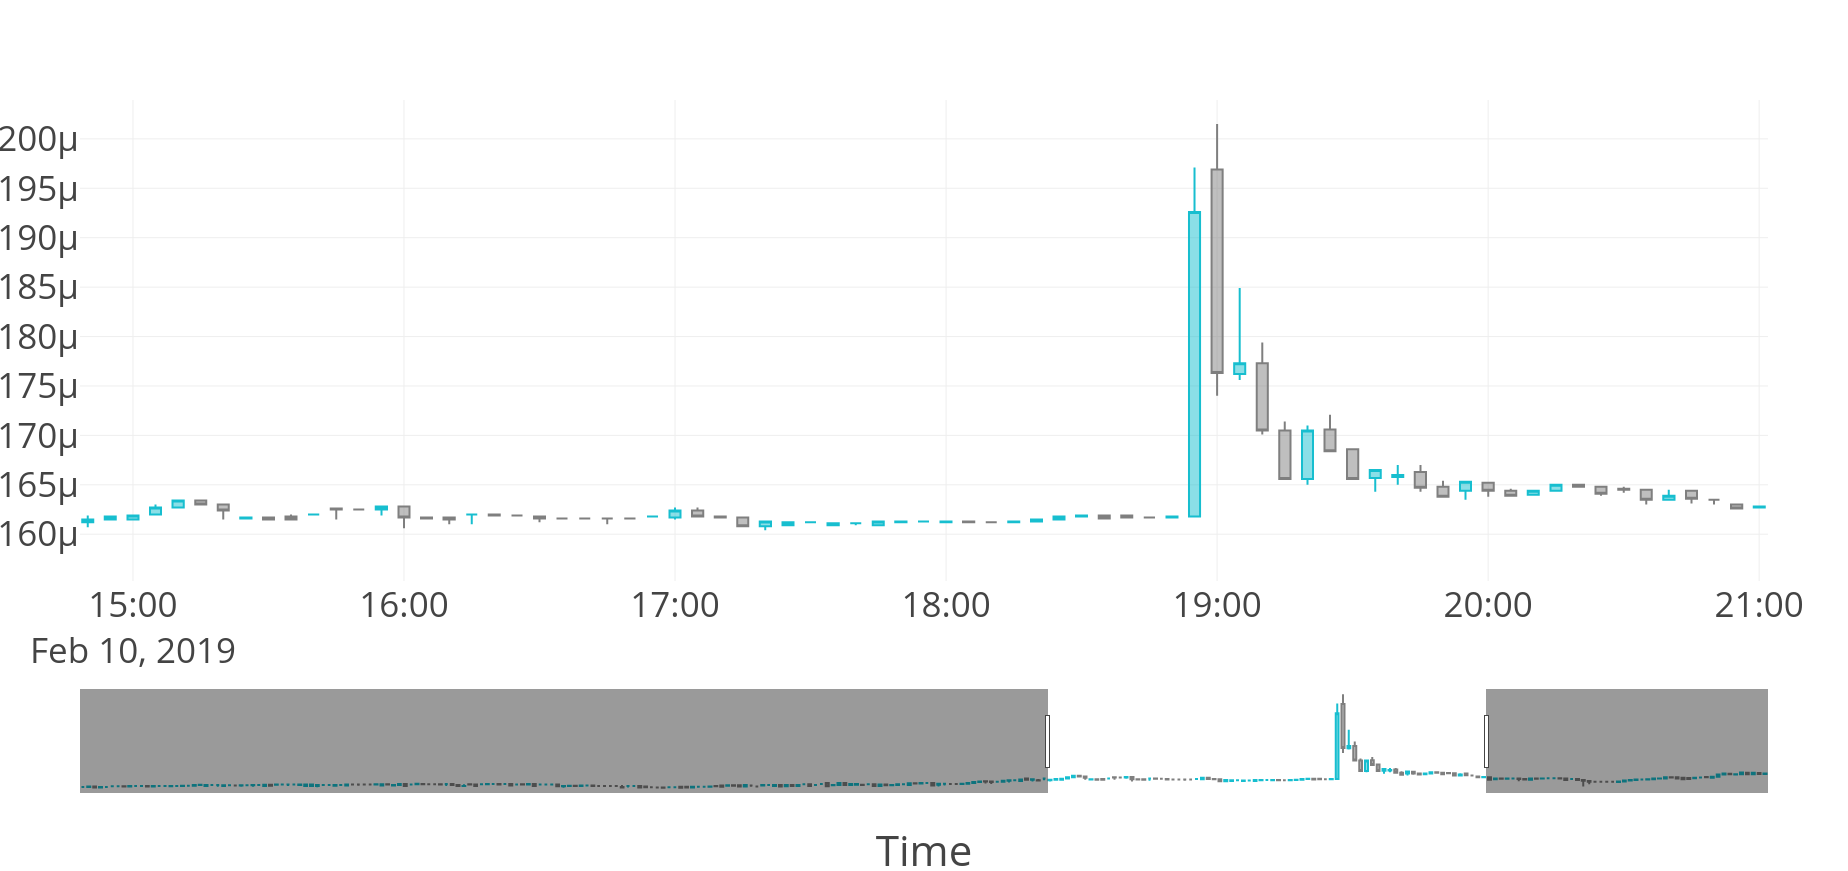
\includegraphics[width=\textwidth]{GXS-BTC.png}
    \centering
    \caption{\ac{pd} organized by the group Crypto Pump Island on 2019-02-10 19:00. The target symbol was GXS/BTC on the exchange Binance.}
    \label{fig:pd-gxsbtc}
\end{figure}

\subsubsection{Characteristics}
Detection of \ac{pd} schemes requires insights in their operations to have the ability to identify patterns that occur during a \ac{pd}. \autoref{tab:pd_characteristics} which is defined by two researchers at the University College London \cite{P&D_anatomy} summarizes some of the fundamental similarities and differences with respect to the target, tactic and timescale of traditional penny stock and cryptocurrency \ac{pd} schemes. It clearly shows that traditional and cryptocurrency \ac{pd} schemes target the same type of markets, but the tactic and timescale differ. The lack of trust among members in the pump groups can explain the short timescale of cryptocurrency \acp{pd}, as they all want their piece of the cake and sell as soon as they profit instead of holding. Spreading of misinformation must happen in real-time because of the short time pressure.

\begin{table}[ht]
    \centering
    \begin{tabular}{l c c}
    \hline
     &\textbf{Traditional} & \textbf{Cryptocurrency}\\
    \hline
     Target   & Low market cap & Low market cap \\
              & Low volume     & Low volume \\
              & Low price      & Low price \\
              & Lack of reliable information & Lack of reliable information\\
              \\
    Tactic    & Misinformation & Real-time\\
              & Privately organized & Public or private group scams\\
              \\
    Timescale & Medium (days to weeks) & Short (Seconds to minutes)\\
    \hline
    \end{tabular}
    \caption[\acf{pd} characteristics]{Characteristics of traditional and cryptocurrency \ac{pd} schemes. (Source: \cite{P&D_to_the_moon}). }
    \label{tab:pd_characteristics}
\end{table}

Using the characteristics, the same two researchers \cite{P&D_anatomy} formulated criterion's that can be helpful when detecting \ac{pd} patterns in exchange data (\autoref{tab:pd_indicators}). The indicators are split into \emph{breakout} and \emph{reinforcers}. The breakout indicators point out patterns that are present during the beginning of a \ac{pd}. And the reinforcers are external aspects to strengthening our confidence in an alleged \ac{pd}. The signs $(+)$ and $(-)$ are a confidential boost; the former denotes an increase while the latter denotes a decrease. The volume and price factors in the breakout indicators are discussed with an estimation window, referring to a collection of previous data points, of some user-specified length~\cite{P&D_anatomy}.

\begin{table}
    \centering
    \begin{tabular}{p{0.33\textwidth} p{0.33\textwidth} p{0.33\textwidth}}
    \hline
    \textbf{Breakout indicators} &\textbf{Real-time indicators} & \textbf{Post-pump indicators}\\
    \hline
    Volume & Has the volume at the current data point been significantly higher than in the estimation window? & Was there a decline in volume after the event window where a pump was detected?\\\\
    Price & Has the price at the current data point been significantly higher than in the estimation window? & Was there a decline in price after the event window where a pump was detected?\\\\
    \end{tabular}
    
    \begin{tabular}{p{0.33\textwidth} p{0.66\textwidth}}
    \hline
    \textbf{Reinforcers} &\textbf{Temporal dimension}\\
    \hline
    Market cap & Is the market cap of the coin relatively low? $(+)$\\\\
    Number of exchanges & Whether the coin is listed on multiple exchanges and the indicators only spike on one $(+)$\\
                        & Whether the coin is listed on multiple and the indicators spike on multiple exchanges (neutral)\\
                        & Whether the coin is not listed on multiple exchanges $(+)$\\\\
    Symbol pair         & Whether the coin is trading for BTC or some other cryptocurrency $(+)$\\
                        & Whether the coin is trading for USD or some other fiat currency $(-)$\\
    Time                & Whether the coin is start on the hour or half hour and last a few minutes$(+)$\\
    \hline
    \end{tabular}
    \caption{Indicators of \ac{pd} per temporal dimension and indicator type. (Source: \cite{P&D_to_the_moon, P&D_anatomy})}
    \label{tab:pd_indicators}
\end{table}
 
\newpage
\section{Machine Learning}
% what is Machine learning? unsupervised and supervised
\ac{ml} is a fast-growing field in computer science, and it refers to the ability to make a computer recognize specific patterns in data using various complex algorithmic models. Selecting a model is tough because it requires a fundamental understanding of the data that suits the model and the model itself to produce first-class results. Models are commonly subdivided into two major paradigms, \emph{unsupervised} and \emph{supervised} learning. In supervised learning, the models require data and prior knowledge of each sample, called \emph{labels} or \emph{ground truth}. The models in unsupervised learning need only data.

% Classification and Regression clustering and


\subsection{Neural Networks}

\subsection{Long short-term Memory}
\cite{lstm}

\newpage
\section{Related Work}\label{sec:related_work}
% Stock Price Manipulation Detection Based on Mathematical Models
An article from ICACI\footnote{International Conference on Advanced Computational Intelligence} 2016, \cite{P&D_stock_price_manipulation} presented a model that detects \ac{pd} schemes on the stock market and did so with $88\%$ accuracy. The article describes how badly \ac{pd} schemes are executed and organized. And from the patterns a \ac{pd} scheme leaves behind, the article proposed mathematical definitions based on level $2$ order book data with a depth of $10$ to generate a training set consisting of buying and sell orders. The researchers implemented a feedforward neural network and trained it with the generated dataset, and achieved an accuracy of precisely $88.28\%$.

% Cryptocurrency Pump Predictions: A novel approach to identifying Pump-and-Dump Scheme
Two students from Standford Unversity recreated the stock market model~\cite{P&D_stock_price_manipulation} and made it compatible with cryptocurrency exchanges in 2017. In their work, they used level $1$ order book data to generate a training set to train a neural network and a Support Vector Machine. They labeled the dataset by identifying \acp{pd} by comparing a market's price movement to BTC. The final test result of their models was $78.13\%$ with Support Vector Machine and $82.5$\% with the neural network. 

The following articles two were recently published, both in late November 2018.

% To the moon: defining and detecting cryptocurrency pump-and-dumps
Kleinberg and Kamps from the University College London\cite{P&D_to_the_moon} defined specific patterns in \acp{pd} and how they differ from the stock market. Also, the article proposed a novel anomaly detection approach based on a set of criteria for locating suspicious transactions patterns on cryptocurrency exchanges. The most balanced parameters for their anomaly detection algorithm resulted in about $1.6$ \acp{pd} per market for a total of $2150$ over $20$ days of data. Moreover, $75\%$ of the alleged pump were to found to have corresponding price dumps.

% The Anatomy of a Cryptocurrency Pump-and-Dump Scheme
Another two researchers in London, but from the Imperial College London, wrote an article that analyzes features of pumped markets and market movement of coins before, and after \acp{pd}.

This article received a lot recognition and attention~\cite{P&D_MIT_crypto, P&D_cointelegraph, } on media platform

in the cryptocurrency community is Xu and Livshits 


% Developed architecture / system design / implementation:
% start with a theoretical approach
% describe the developed system/algorithm/method from a high-level point of view
% go ahead in presenting your developments in more detail

\chapter{\project's Design}\label{ch:design}\glsresetall
% Our application is building entirely on decision making. If it seems like a \ac{pd} is coming up, buy, then sell on profit. Otherwise, wait for a \ac{pd}. Simple, yet effective if and only if the application can make accurate predictions. Our prediction algorithm needs to either detect \acp{pd} before it happens or exactly when it begins, because of the period where \ac{pd} peak span from seconds to max $10$ minutes as described in \autoref{sec:pd}. Are we too late with buying assets we may end up buying at or right before the peak which will result in a substantial loss because of the forthcoming dump. However, if we can manage to purchase assets just a few seconds in or before the \ac{pd} starts we can profit well by selling only a short time later when the coin peaks.

% For the application to have the ability to make accurate predictions, we need to carefully define a suitable algorithmic model that fits currently existing data to reverse engineer \acp{pd}. We find two paradigms \emph{financial} and \emph{\ac{ml}} as appealing fields for finding suitable algorithmic models. We encounter some problems in the field of finance, typically, financial institutions do not share their algorithms for competitive reasons, and we can not either find any models that are compatible for detecting \ac{pd} in real-time on cryptocurrency exchanges. We believe that using \ac{ml} to detect \acp{pd} is currently the optimal solution, and to reinforce that assumption, a recent PwC\footnote{Price Waterhouse Coopers is the largest network of accountants, lawyers and advisors, and deliver services within audit, consulting and tax.} study found that over the next two to three years \ac{ml} are the single most crucial technology impacting the finance function~\cite{pwc} as \ac{ml} models seem to excel financial models.


% Supervised learning problem
% binary classification problem
% Pump are anomalies
% choosing a model

% Moving on with \ac{ml}, we can define detection of \ac{pd} as a supervised \emph{binary classification} problem, \ac{pd} or not \ac{pd}. As with every supervised problem we need data that is labeled which are struggling to get.


% Our application only requires the knowledge of the pump part in a \ac{pd} to function. Our application wants to buy before or at the beginning of a pump and sell when the coin peak.

% Our application only requires the knowledge of the pump part in a \ac{pd}, as our application want to buy before or at the beginning of a pump and sell when the coin peak. We can ignore the dump part because it do not affect the decision made by our application. We can define this as a \emph{binary classification} problem, pump or not pump, or from our application perspective buy or sell.

% \acp{pd} are a common price manipulation scheme one observe on cryptocurrency exchanges, but in vast amount of existing data that exchanges produce a \ac{pd} is an \emph{anomaly}. It exist way more regular data than \ac{pd} data. This becomes problem when we want to  create a dataset containing regular data and \ac{pd} data because of the huge imbalance between the two classes, and \acp{pd} are rare entities hence it is also challenging to obtain a significant amount of \acp{pd} required to train a \ac{ml} model.

% Choosing a \ac{ml} model primarily depends on the nature of the input data. Input data can be broadly classified into sequential (e.g., voice, text, music, time series, protein sequences) or non-sequential data (e.g., images, other data)~\cite{dl_anomaly}. Cryptocurrency sources produce sequential data, more specifically \emph{time series} data. Time series data are linearly ordered sequence of values of a variable at equally spaced time intervals~\cite{stat_handbook}. 

% Anomaly detection in sequential data has attracted significant interest in the literature due to its applications in a wide range of engineering problems. \ac{lstm} neural network based algorithms for anomaly detection have been investigated and reported to produce significant performance gains over conventional methods  (Ergenet al. [2017]).

% Supervised anomaly detection techniques are superior in performance compared to unsupervised anomaly detection techniques since these techniques use labeled samples (G ̈ornitz et al. [2013]).  Supervised anomaly detection learnsthe separating boundary from a set of annotated data instances (training) and then, classify a test instance into eithernormal or anomalous classes with the learned model (testing).

% Moreover, the performance of deep supervised classifier used an anomaly detector is sub-optimal due to class imbalance (the total number of positive class instances are far more than the total number of negative class of data)~\cite{dl_anomaly}.

% Labels indicate whether a chosen data instance is normal or an outlier. Anomalies are rare entities hence it is challenging to obtain their labels~\cite{dl_anomaly}.
TBW
\section{Overview}
We are modeling \project as a \ac{ml} pipeline, but with some few extensions. It is designed to extract raw data from different cryptocurrency sources and transform it into valuable features in order to classify \acp{pd}. The term \ac{ml} pipeline can be misleading as it implies a one-way flow of data when some elements in the pipeline are cyclical and iterative where every iteration intends to improve the accuracy of the model~\cite{ml_pipeline_3}. Some of the advantages a pipeline provides is~\cite{ml_pipeline_2};

\begin{figure}[ht]
    \centering
    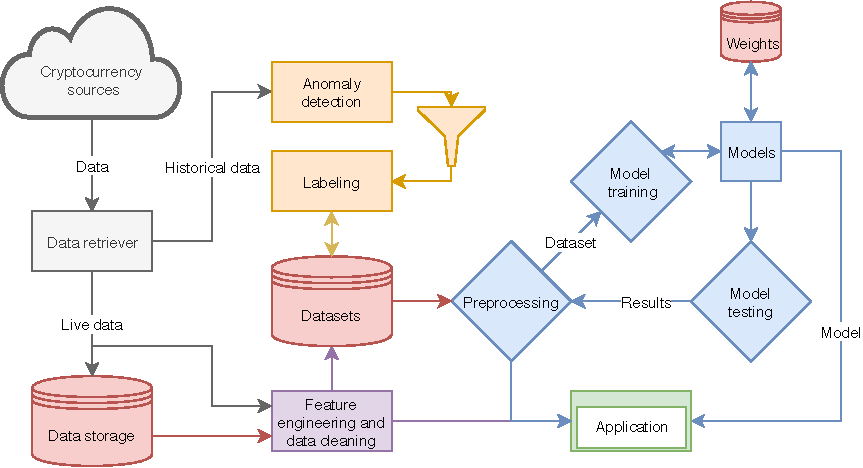
\includegraphics[width=\textwidth]{overview.pdf}
    \caption{Architectural overview of \project}
    \label{fig:overview}
\end{figure}

The first step in the pipeline pulls data from various cryptocurrency sources. The data is mostly incomplete and lacks behaviors or trends making it currently pointless to train a model with. This process is tedious because sources tend to have different request rates, \acp{api}, and the data can have various formats like \ac{json} or \ac{xml}.

The next step branches the retrieved data in two, live and historical data. Since we are trying to detect \acp{pd} in real-time we need to store live data continuously. When captured a compelling amount of \acp{pd} in the stored live data, we use an anomaly detection algorithm~\cite{P&D_to_the_moon} to detect \ac{pd} in the gathered live data. This algorithm is not compliant with live data, so we need to pull aggregated historical data that span throughout the collected live data. As previously mentioned, anomaly detection algorithms tend to have a high false positive rate. Thus, we need to remove these false positive and keep the true positive manually.

The input data ultimately determine the performance of a \ac{ml} deep learning model~\cite{mike_voets}, so training a model with the raw gathered live data is ineffective. Hence, we need to define new convenient dataset containing features created by processing the collected live data; this is a highly critical process and will later determine the classification performance of the deep learning model. The gathered live data also need to go through a cleansing process as it most likely does not contains relevant \ac{pd} information.

With filtered anomalies containing \ac{pd} and a dataset, we can create a labeled dataset and train our model. Obtaining good classification results depends, as mentioned, on the features, but also how we decide to pre-process the dataset. Typical pre-processing strategies include dimensionality reduction and normalization. Having a labeled pre-processed dataset we can finally begin to the train the deep learning model, this a cyclical and a long process, as it requires many trial and error attempts to find the optimal weights for the model. In each cycle, we store the model's weights because it is not always the case that each iteration will improve the classification performance of the model.

For applications to utilize \project, they need to select a model and let live data flow through the same processing stages as the dataset that was used to train the model.

\section{Internal Components}
TBW

\subsection{Retrieving Data}
Every problem that is solved using \ac{ml} requires data, the more, the merrier when training a model. As previously mentioned, cryptocurrency sources like exchanges produce time series data containing, e.g., price and volume of a coin. Such data is continuously produced in a restricted amount with proportion to time.

Since we want to detect \acp{pd} on exchanges in real-time, the nature of the data we want to make classifications on is  live fine-grained data so that the model can detect them as early and accurate as possible. Aggregated historical data is too coarse-grained because exchanges generally only allow a discrete time interval selection of data where the smallest is typically one minute. The duration where they start to where they peaks varies from a few seconds to max ten minutes~\cite{P&D_MIT_crypto, P&D_to_the_moon}, and the ability to make accurate predictions with one-minute data is questionable.

Training a model in real-time by pulling data is impractical because we do not have the \acp{pd} labels then, and sources can only produce a limited amount of data at a time which will create a bottleneck of data supply to the model. To cope with these problems, we have to pull and store current live data continuously; this is an endless dreary process for we have to wait weeks until we have "captured" enough \ac{pd} events in our collected data to start training. If anything fails, we may have to start all over again as we are missing out on trends, which results in noisy data.

From the reinforcers field in \autoref{tab:pd_indicators}, to reverse engineer \acp{pd}, we have to fetch data from various sources. An exchange alone does not produce data regarding a coin's capitalization, nor a coin's price on a different exchange. Other sources than exchanges produce such metadata of coins, while exchanges only produce internal trading data.

\subsubsection{Master Slave Approach}
We shape our data retriever like a master/slave model.\autoref{fig:ms} is an example that illustrates our data retriever with a master and its three data pulling slaves. Each slave in our data retriever is assigned a source that can be, e.g., an exchange. The communication between slaves and the master is intuitive. The master broadcasts a pull signal to the slaves, and they pull the data from their assigned source, then the master gathers the data from them and parses it, and augments it to a sample. Each sample the master generate gets stored. This procedure takes effect in a fixed interval for obtaining clean time series data, such that each sample's time gap is equal. The advantages and disadvantages of this structure are:

\begin{figure}[ht]
    \centering
    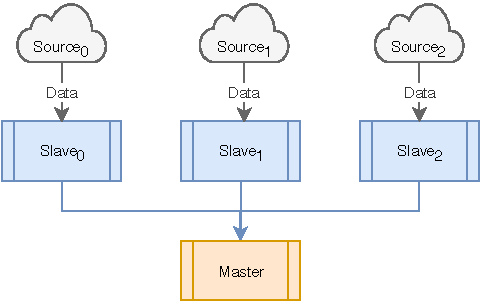
\includegraphics[width=0.8\textwidth]{ms.pdf}
    \caption{Master/slave structure}
    \label{fig:ms}
\end{figure}


\textbf{Advantages}
\begin{enumerate}
    \item \emph{asynchronous requests} - Each pull-broadcast issued by the master starts a series of requests in parallel from the slaves. Thus, each request is roughly issued simultaneously making features in a sample equally spaced in terms of time.
    % Frequently fetching of data from the internet is an \ac{io} bound problem, and are typically solved with multiprocessing or concurrency if needed. If we choose a single process to make synchronous requests, a bottleneck could have occurred, and requests would be issued separately that results in various time gap among features in each sample.
    
    \item \emph{removes race condition} - Since each data sample is \emph{sequentially} written to disk by the master, a race condition can not take place. 
    % If the slaves processed their data and wrote to the same location, at some point in time, a race condition would take place and corrupt the data. Even though these race conditions are rare, anything that can happen will happen, Murphy's law.
    
    \item \emph{horizontal scaling} - Scales by adding slaves instances~\cite{ms_hor}; there is no upper limit of them. In the end, the bottleneck is the master if its have too many of them to communicate with.
    
    \item \emph{faulty slave tolerance} - If a slave crash, the data retriever is still progressing, but it also results in partial storage of data. Hence, this will most likely corrupt a good portion of the collected data.
\end{enumerate}

\textbf{Disadvantages}
\begin{enumerate}
    \item \emph{\ac{spof}} - If the master crash, the slaves will not retrieve data.
\end{enumerate}

\subsubsection{Collecting Trading Data From Multiple Markets}
Previous work in detection of \acp{pd}~\cite{P&D_to_the_moon}, estimated that $1.6$ \acp{pd} is carried out daily per market, this raises several problems. First, multiple exchanges have the same market, and we can not know which exchange they target unless we have prior knowledge from their \ac{pd} group. Second, gathering data from a single market is inadequate, the data retriever would with an estimate captured $48$ \ac{pd} occurrences, if it gathered every \ac{pd} event on a single market in a whole month. Training a model with $48$ instances is insufficient. 

Therefore, we collect data from all the markets from a single exchange to make sure we obtain as many \acp{pd} as possible. Inbefore doing that, we need to make a considerable assumption, that is, \acp{pd} pattern remain the same across markets. Otherwise, if it does not, we may run into trouble when training our model by having too few samples with various patterns. By training a model using data from all the market makes it general, allowing it to adapt to new markets as the exchange issues them. 

The reason we are targeting a single exchange is that they have different \acp{api}, although the data they provide are mostly identical, in some way, each exchange does stand out by providing some unique data. Thus, we can utilize every piece of information we receive from an exchange without the concern of making it compatible with data existing on other exchanges.

\subsubsection{Feature Description}
From the \ac{pd} indicators described in \autoref{tab:pd_indicators}, we define a set of features described in \autoref{tab:features}, we believe that these features contains the necessary information for a model to detect \acp{pd}. We fetch all these features for each market.

Some features like a coin's capitalization are available at \href{https://coinmarketcap.com/}{CoinMarketCap}, while trading data like order book and \ac{ohlcv} values are available at exchanges. A specific feature that is challenging to attain is aggregated \ac{ohlc} values from multiple exchanges, as this requires us to request multiple exchanges simultaneously and aggregate the data.

\begin{table}[ht]
    \centering
    \begin{tabular}{p{0.30\textwidth} p{0.70\textwidth}}
        \hline
        \textbf{Feature} & \textbf{Description}\\
        \hline
        \ac{ohlcv}                      & Latest \ac{ohlcv} values.\\
        \hline
        \ac{ohlcv} multiple exchanges   & Aggregated \ac{ohlcv} values from multiple exchanges.\\
        \hline
        Order book                      & Level $1$ (aggregated price and volume) order book with a depth of $5$.\\
        \hline
        Order book imbalance            & The imbalance between bids and asks orders and quantity.\\
        \hline
        Coin capitalization ratio       & Coin capitalization ratio.\\
        \hline
        Volume traded                   & Base and quote volume traded for the last $24$ hours.\\
        \hline
        number of trades                & Number of completed trades for the last $24$ hours.\\      
        \hline
        bid and ask price               & Best bid and ask price for the last $24$ hours.\\
        \hline
        bid and ask volume              & Best bid and ask quantity for the last $24$ hours.\\
        \hline
        Average price                   & Average price for the last $24$ hours.\\
        \hline
        symbol-pair exchange rate       & The rate of how many exchanges that lists the symbol-pair.\\ 
        \hline
        Time                            & Unix timestamp.\\
        \hline
    \end{tabular}
    \caption[Features description]{Feature description}
    \label{tab:features}
\end{table}


\newpage
\subsection{Preparing Data}\label{sec:prep}
In practice, it has shown that data cleaning and preparation takes approximately $80\%$ of the total data engineering effort, as it requires solid domain knowledge of the subject. Data preparation is, therefore, an important research topic. Data preparation comprises those techniques concerned with analyzing raw data to yield quality data, mainly including data collecting, data integration, data transformation, data cleaning, data reduction, and data discretization~\cite{zhang2003data}.

For the reason that we fetch data from multiple sources and markets to create a general model, we must prepare the data for it. Since markets are distinct, they surely have various numerical values, such as different trading price and volume, and making predictions with these numerical values that fluctuate from market to market is nonviable. E.g., assume a \ac{pd} occurs on a coin with a low cost, and the price is increasing with $300\%$. Despite the high increase and profit, the coin is still almost worthless compared to other expensive coins, and the model do not distinguish between markets, all markets are equally weighted. It looks at each feature as "more" or "less" of something. Thus, we must transform all these numerical values into some other values.

\subsubsection{Data Cleansing}
Data cleaning, also called data \emph{cleansing} or \emph{scrubbing} deals with detecting and removing errors, inconsistencies, and unproductive features from data in order to improve the quality of data~\cite{data_cleaning}.

Fetched data from exchanges includes additional features not defined in \autoref{tab:features}. These features do we have to remove as they probably adds nothing of valuable knowledge. Instead, they increase the number of dimensions and makes the data more complex.

Markets with little or no activity may have intervals containing \emph{zero-data}, e.g., if no investors have bought or sold assets in a specific interval, exchanges tend to set the trading values to zero. These zero-values create significant jumps/spikes in the trend which we must fix; otherwise, they disrupt the data. Besides, having zero-data does not make any sense, if the price is recorded to be zero, then it means that coin is free which it is not.

We substitute every value that is zero by linear interpolate each of them. Linear interpolation involves estimating a new value by connecting two adjacent known parameters with a straight line~\cite{interpolate}. These two known parameters are non-zero values that are adjacent on each side of the zero-value. Thus, we form the following \autoref{eq:interpolation} with the known parameters $(x_1, y_1)$ (previous non-zero value) and $(x_2, y_2)$ (next non-zero value), $y$ is the new value for some zero-value in point $x$.

\begin{align}\label{eq:interpolation}
    y = y_1 + (x - x_1) \frac{y_2 - y_1}{x_2-x_1}
\end{align}

\subsubsection{Feature Engineering}
Feature engineering is the process of using domain knowledge of the data to create features that make \ac{ml} algorithms work. Feature engineering is fundamental to the application of machine learning and is both challenging and expensive, but when done correctly, it can result in wonders~\cite{feature_engin}.

\begin{displayquote}
    \begin{em}
        "Feature engineering is the art part of computer science" - Sergey Yurgenson
    \end{em}
\end{displayquote}
 
\subsubsection{Processing Order Book}
As previously mentioned in \autoref{sec:pump_groups}, \ac{pd} organizers invests in the market before the \ac{pd} without raising the price. We believe that the order book in said market oscillates in before the pump, and especially during the pump. Therefore, we calculate an imbalance between sell and bids order; this is a multidimensional problem considering an order book contains both a list with prices along with its volume as we saw in \autoref{tab:order_book}. \autoref{eq:imbalance} reduces this multidimensional problem to a single value with equal weight to price and volume. $p$ and $v$ is respectively the lists with prices and volumes, and the annotations $a$ and $b$ denotes asks and bids orders. If \autoref{eq:imbalance} yields a value between $(0,1)$, then it weigh more bidders, if it yields a value between $(1, \infty]$, then askers, and $1$, there is an equal weight of bidders and askers.

\begin{align}\label{eq:imbalance}
    imbalance = 
    \frac{
    \begin{bmatrix}
        p^a_1 \\
        \vdots \\
        p^a_n
    \end{bmatrix}
    \cdot
    \begin{bmatrix}
        v^a_1 \dots v^a_n
    \end{bmatrix}
    }{
    \begin{bmatrix}
        p^b_1 \\
        \vdots \\
        p^b_n
    \end{bmatrix}
    \cdot
    \begin{bmatrix}
        v^b_1 \dots v^b_n
    \end{bmatrix}
    }
    = \frac{\langle P_a, V_a \rangle}{\langle P_b, V_b \rangle}
\end{align}

\subsubsection{Processing Trading Data}
We process trading data such as price and volume by calculating the percentages of change, which makes each market comparable and eliminates the need for the model to adjust to prices. For example, if ETH is up \$$10$ from a starting value of \$$100$, and ADA is up \$$5$ from a starting value of \$$50$, then both coins are up $10$\%.

We define the function $pct$ to calculate the percentage of change. It calculates the percentage change in point $x$ concerning a previous value $v$ with a time lag $\gamma$. We consider $x$ and $v$ to be a single value like the price or volume, while $\gamma$ indicates moving backward in time from point $x$. We must be vigilant when using this technique, if the data contains values that are zero, we might perform a zero-division that can clutter with the data unpredictably. However, since we scrubbed the data first and removed this zero-values, this should not be a concern.

\begin{align*}%\label{eq:pct}
    pct(x, v_\gamma) = \frac{x - v_\gamma}{x}
\end{align*}

Differentiating and take the tangent line instead could be a solution, but since we are fetching data from multiple markets, the tangent would always favor expensive markets. Using the tangent would be illogical when \ac{pd} organizers tend to target low-cost markets.

\subsubsection{Processing Time}
According to \cite{P&D_anatomy}, the time is essential when classifying \acp{pd}, as they are typically executed at the hour (6:00, 7:00, etc.) because organizers usually does not choose a random time.

\begin{equation}\label{eq:unix_time}
    x_\delta(x_{\textbf{unix}}) = \frac{x_\textbf{unix}\mod 3600}{3600}
\end{equation}
\myequations{UNIX timestamp scaling}

\begin{align}\label{eq:gaus}
    t(x_\delta, \mu, \sigma) &= \frac{1}{\sqrt{2\pi\sigma^2}} e^{-\frac{x_\delta-\mu}{2\sigma^2}}, \quad \text{where}
    \begin{cases}
    \mu = 0.5 \\
    \sigma = 0.1 
    \end{cases}
\end{align}
\myequations{Data preparation - Time}

Data retrieved from sources are getting timestamped, and we can take advantage of these timestamps to check whether data was generated at the hour or not. The function $x_\delta$ transforms a Unix\footnote{unix timestamp is a way to track time as a running total of seconds.} timestamp to a value in the interval $[0, 1)$. The closer $x_\delta$ is to the margins, the closer the time is at the hour, but since $0$ and $1$ symbolizes the same, we have to process it further before we can use it as a valuable feature.

We define a Gaussian distribution function $t$ with the parameters $\mu=0.5$ and $\sigma=0.1$ which creates the graph illustrated in \autoref{fig:unixtime}. The graph shows when given $t$ a $x_\delta$ close to $0$ or $1$ (6:00, 7:00, etc.), $t$ returns a value close to $0$, but when given $0.5$ (6:30, 7:30, etc.) it returns a value close to $4$. $t$ demonstrate that we can separate data by how close it was generated at the hour. Also, we can always tweak $\sigma$ to adjust the width of the wave. Adjusting the wave allows us to be more strict, the wider the curve, the more strict.

\begin{figure}
    \centering
    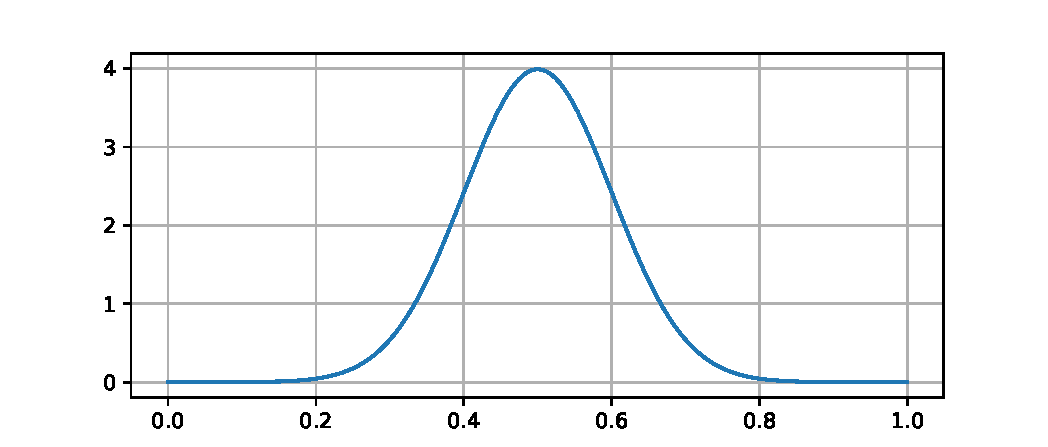
\includegraphics[width=\textwidth]{time.pdf}
    \caption{Gaussian distribution}
    \label{fig:unixtime}
\end{figure}

\subsection{Collecting Pump-and-Dumps}
Manually collecting \ac{pd} events from chat applications to label our collected data, seems infeasible in the long run — even tough Livshits and Xu \cite{P&D_anatomy} hand-picked $220$ pump-events from July to November in 2018 from $358$ different Telegram groups to train a Random Forest. They still did miss out on plenty of other executed \ac{pd} schemes as there are numerous of other chatting applications and private organizers~\cite{blockonomi}. Also, searching for \ac{pd} events is a time-consuming process, and incorrect labeling occurs when we lack membership to all of \ac{pd} groups, which results in more mediocre prediction capacity~\cite{label_noise}. We also have to be aware if a \ac{pd} was successfully executed or not; labeling failed attempts as positive only contributes to label noise. Instead of manually collecting \acp{pd} from groups in chatting applications, we believe that it is possible to hand-pick \acp{pd} by \emph{reasoning abductively} with the help of an anomaly detection algorithm to pinpoint suspicious time intervals in historical data.

The anomaly detection algorithm identifies local \emph{contextual anomalies} based on fixed recent history called a \emph{sliding time window}. Contextual or conditional anomalies are abnormal data points within a specific context and are prevalent in linearly ordered data called \emph{sequence data}~\cite{anomaly_survey}. A sliding window is a period that stretches back in time (lag factor) from the present containing events at specified intervals. The event intervals can overlap with each other, or they can be disjunct. As events exceed the lag factor, they fall out of the sliding window, and they are no longer matching against the rules applied to the sliding window~\cite{redhat}. With a sliding window, we can compare values in a given period~\cite{P&D_to_the_moon}, contrary to using single values, which not yield much information alone in sequence data.

The anomaly detection algorithm is proposed by Kleinberg and Kamps \cite{P&D_to_the_moon}, which is inspired by previous research in \ac{dos} attacks~\cite{dos}. It is a threshold based technique to find a suspicious increase in price and volume of a coin. If the price and volume in a specific interval are higher than some threshold, then the interval is flagged anomalous and worth further investigation.

\subsubsection{Price Anomaly}
We compute the price anomaly threshold by a simple moving average $\mu_\gamma^p$ of \ac{ohlcv} values denoted $x$ with a lag factor $\gamma$ multiplied with a given percentage increase $\epsilon_p$. We consider $x$ and $\gamma$ as \ac{ohlcv} objects, and $x-\gamma$ indicates moving backwards in the sliding time window by a factor of $\gamma$~\cite{P&D_to_the_moon}. If the highest registered price in $x$'s period is greater than the computed threshold, we flag the period as anomalous.
\begin{align}
    \mu_\gamma^p(x) &= \frac{\sum^x_{i=x-\gamma} x_{close}}{\gamma}\\
    price\_anomaly(x)&=
    \begin{cases}
        True  & \text{if $x_{high} >    \epsilon_p \cdot \mu_\gamma^p(x)$}\\
        False & \text{otherwise}
    \end{cases}
\end{align}

\subsubsection{Volume Anomaly}
Calculating the volume anomaly threshold is almost identical to the above, we are only substituting $x_{closing}$ and $x_{high}$ with $x_{volume}$, which form the following expression.
\begin{align*}
    \mu_\gamma^v(x) &= \frac{\sum^x_{i=x-\gamma} x_{volume}}{\gamma}\\
    volume\_anomaly(x)&=
    \begin{cases}
        True  & \text{if $x_{volume} >    \epsilon_v \cdot \mu_\gamma^v(x)$}\\
        False & \text{otherwise}
    \end{cases}
\end{align*}
\myequations{Anomaly - Volume}

\subsubsection{Filtering Anomalies}
Anomaly detection algorithms, in overall, have a high false alarm rate~\cite{grill2017reducing}, which makes them difficult to use. Since we want to use these anomalies we collected to train a model with, it is, with high importance, to remove false \acp{pd}. Otherwise, training a model with false \acp{pd} will make the model perform worse, and results in a high occurrence of false positives which is already a problem. Therefore, we manually remove all the false positives anomalies, but removing them requires prior knowledge of \acp{pd}, which we do not have.

Since the anomaly detection algorithm checks whether a \ac{pd} occurred in a specific interval, and not exactly when. We visualize one-minute \ac{ohlc} from that interval in a chart, by plotting these values we can compare them to a few charts containing real \ac{pd}. Additionally, a market's capitalization, if the pairing coin is BTC, or how many exchanges that list the market, can be helpful when filtering \ac{pd}. E.g., if the anomaly detection algorithm flagged a suspicious interval in the ETH-BTC market, and it visually looks like a \ac{pd}, then it still would with a high likelihood not be a \ac{pd} because ETH is the coin with second highest capitalization~\cite{coinmarketcap_eth}, and that would break the pattern where the organizers target coin with low capitalization. Further helpful characteristics regarding \acp{pd} is described in \autoref{tab:pd_characteristics} and \autoref{tab:pd_indicators}.

\subsubsection{Labeling Pump-And-Dumps}
With the new features generated by the collected data and filtered anomalies containing \acp{pd}, we can label the new features and define a dataset, but first, the filtered anomalies still contains intervals where \acp{pd} occurred, and not exactly when it was executed. So, we need to precisely define where every \ac{pd} started end ended, before labeling.

Because the purpose of \acp{pd} is to raise the price of an asset, makes us believe that, where the price change is highest in an interval, that is where the \ac{pd} peaked. If we have the peak of a \ac{pd}, we can search from the peak and down the descending slopes on each side of it. Left side, pump. Right side, dump. From each side we search until the change in price is equal or smaller than $0$. Finally, when have defined the start and end of every \ac{pd}, we label all the new features positive where there are \acp{pd}, and negative otherwise.

\subsection{Deep Learning}
This section describes the model we use to detect \ac{pd}, and how we process data, trains the model, and which metrics we should use to evaluate the model. These steps are an iterative process, where each iteration tend to improve the model.

\subsubsection{Preprocessing}
Before training a model with the generated dataset, we transform it by \emph{normalizing} Since the features in our dataset have various scales, some percentages, some other numerical values, then, a common technique do is to \emph{normalize} the input data. Normalization creates new values from the dataset, but still maintain the general distribution and ratios in the source data while keeping values within a scale applied across all used features~\cite{normalize_data}. Also, normalization, in some cases, improves the performance of the model~\cite{normalize_google}, and accelerate convergence speed resulting in shorter training time~\cite{sola1997importance}.

There are several ways to normalize data, and which normalization technique one use may have an impact on the performance of the model. Since \acp{pd} are anomalies, some features like percentage change in price and volume will make them look like outliers in the data. A traditional method called \emph{min-max} normalization is repeatedly used in detection of outliers~\cite{campos2016evaluation, goldstein2016comparative}. This technique provides a linear transformation of the data~\cite{panda2014smoothing}, allowing us to keep the distance ratio, and it scales every value into the range $[0,1]$.

\begin{align}\label{eq:minmax}
    x_{ij}' = \frac{x_{ij} - \min(x_j)}{\max(x_j)-\min(x_j)} 
\end{align}

\autoref{eq:minmax} is the min-max normalization formula for a coefficient $x_{ij}$, where $x_j$ is a column in a dataset with row vectors.

\subsubsection{Model}
The basic model type we use to detect \ac{pd} is a \ac{rnn} \ac{lstm} network. This network contains \ac{lstm} cells in the hidden layer because we want the cells to have an internal state (memory) to remember the trend in data. We modeled the detection of \acp{pd} as \emph{binary classification} problem, \ac{pd} or not \ac{pd}. So, we only need a single perceptron in the output layer. \autoref{fig:lstm} illustrates the model.

We can build a more complex network with multiple layers containing \ac{lstm} and perceptron cells, but with a deeper network, the time it takes to train increases simultaneously as it is harder to find the optimal parameters of the network. 

\begin{figure}[ht]
    \centering
    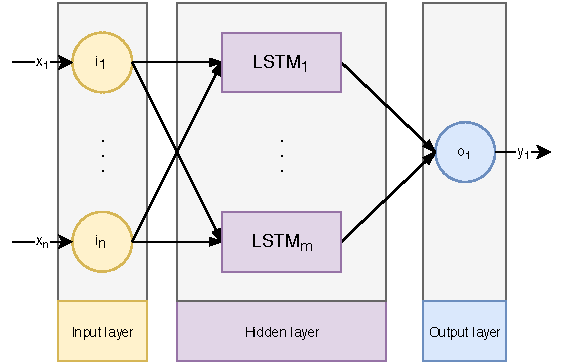
\includegraphics{lstm.pdf}
    \caption{Structure of the model}
    \label{fig:lstm}
\end{figure}

\subsubsection{Training}
Before we start to train our model, we have to split the dataset into two sets, a training set, and a test set. The training set will we use to train the model, and the test will we use to evaluate the model. There is also a validation set that is used to fine-tune the hyperparameters during the training, but since there are so few \ac{pd} samples, we choose to avoid using a validation set and use those \ac{pd} samples we have to train our model and evaluate it.

As previously mentioned, \acp{pd} are anomalies, and that results in a significant class imbalance between positive and negative samples, which, when trained will make the model to overfit to the negative class and more or less ignore the positive class, it entirely depends on the distribution of them. Also, the academia is split concerning the definition, implication and possible solutions to this problem~\cite{tw_imbalance_2} making it currently ambiguous how to properly deal with it.

\begin{figure}[ht]
    \centering
    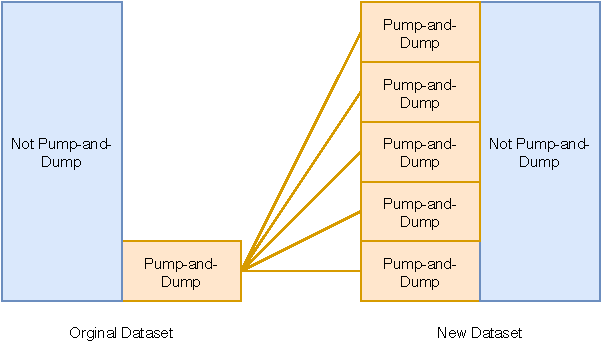
\includegraphics{oversampling.pdf}
    \caption{Oversampling (source\cite{tw_imbalance})}
    \label{fig:oversampling}
\end{figure}

We believe that we can solve our imbalance problem by using a technique called \emph{oversampling}, which \autoref{fig:oversampling} illustrates. Oversampling gathers all the samples from the minority class and duplicates them until the amount is approximately equal to the majority class. There is also a technique called \emph{undersampling}, that select random samples into a subset from the majority class until the size is equal to the number of samples in the minority class, but by using the oversampling technique, we can train our model with the whole dataset. With a balanced dataset, we can finally train our model.

Sometimes, depending on the size of the dataset and number of epochs, training a model takes a really long time. Thus, after each training, we store the model and all its weights and other internal parameters.

\subsubsection{Evaluation}
After the training phase, we evaluate the model by classifying all the samples in the test dataset. The metrics, \emph{precision}, \emph{tp-rate}, and \emph{fp-rate} are probably the most important metrics to optimize when it comes to detection of anomalies. Sometimes, finding the best parameters is done by multiple trials and errors attempts. Adjusting the parameters like number of, hidden layers, cells, and epochs, might improve said metrics. Also, shuffling samples may improve the model as we train with a few numbers of original \acp{pd} samples.

\section{Stitching it all together}
Till now, in this chapter, we have described each component in \project. As we mentioned in \autoref{ch:background}, when we have trained a model and are satisfied with how it performs, we can be fed the model with real-time data, and it will classify whether the given data is a \ac{pd} or not. This allows us to dismiss numerous components which are not needed anymore. They only need to be present during the training phase. So we can divide \project into two phases, a training phase, and a deployment phase. In the training phase, \project entirely depends on all the components. In the deployment phase, there are only a few necessary components.

\subsection{Deployment Phase}
In the deployment phase, we only need a handful component, these components are in \autoref{fig:pipe}. The first component, the retriever function precisely like described above, it fetched data and pushes it further down the pipeline, but it is essential that it fetches the same type of data from the same sources. The next two stages are different, as they need to remain a state from the training phase. In the feature engineering stage, we have to use the same parameters in the cleansing and feature engineering method. Otherwise, the model will classify data that is not what it trained with. Also, in the processing stage, it is highly essential that we normalize the input data with the precisely same parameters as we used with the training set. Else, the input data is scaled the inconsistent parameters, which with result in more misclassification.

The application needs to select a model that was generated during the training phase. With both a trained model and processed real-time data, the application can with ease predict in real-time, whether if the input data is a \ac{pd} or not.

\begin{figure}[h]
    \centering
    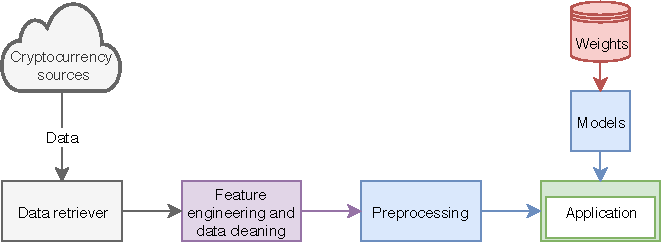
\includegraphics{pipe.pdf}
    \caption{Deployment pipeline}
    \label{fig:pipe}
\end{figure}
%XXX Since design will focus on each component, this section can mirror the previous chapter, but instead of high level overview, describe how you implemented the description from the design chapter, programming language, libraries etc.

% Python
% Data collection - ccxt, binance, coinmarketcap
% historica data - anomaly detection - matplotlib -ohlcv - pandas - numpy 
% labeling - matplotlib - ohlcv - anomaly d
% generating dataset

\chapter{Implementation of \project}\label{ch:implementation}\glsresetall
This chapter describes the implementation of \project. It first, define which programming language and modules we use during the implementation. Then it details how we implement each component.

We implement the system in the programming language \href{https://www.python.org/}{Python}, which we is a powerful high-level scripting language that is excellent for building prototypes and conducting experiments. It has an extensive and superb standard library, but it also has an active community which provides specialized software that implements various protocols, \acp{api}, etc. It has roots in multiple programming paradigms like procedural, object-oriented, and functional. In recent year, it has climbed to the very top of being the most popular programming language according to PYPL\footnote{Popularity of Programming Languge}~\cite{pypl_python}.

Python has an interpreter, a program that executes the code. Each python interpreter has a \ac{gil}, which is a mutex that protects access to the Python object, preventing multiple threads from executing Python bytecodes at once. This lock is necessary mainly because CPython's memory management is not thread-safe~\cite{python_gil}. Because of the \ac{gil}, a single interpreter cannot execute threads in parallel. To run parallel code in python, we must launch multiple interpreters. If we refer to a process, we refer process with its own interpreter, and we use a thread, then we refer to a thread that's running within an interpreter.

The modules we use are all available from PyPI\footnote{Python Package Index}, a python software repository, and they are all easily installable by using PyPI's package installer pip. The following modules we take advantage of are:

\begin{itemize}
    \item \textbf{ccxt} - package containing a uniform \ac{api} for supporting numerous exchanges.
    \item \textbf{keras} - high-level deep learning network \ac{api}.
    \item \textbf{numpy} - fundamental scientific computing module.
    \item \textbf{pandas} - library containing data structures and data analysis tools.
    \item \textbf{matpotlib} - plotting library.
    \item \textbf{time-series} - module for working with time-series data.  
    \item \textbf{scikit-learn} - tools for data mining and analysis.
    \item \textbf{python-binance} - Python implementation of the exchange Binance.
    \item \textbf{CoinMarketCapAPI} - Python implementation of the cryptocurrency tracking site CoinMarketCap.
\end{itemize}

\section{Data Retriever}
%% MS
% Master
% Slaves - polymorphism
% Dataframe
We implement our data retriever like a master/slave architecture in Python as we described in \autoref{sec:ms}, where the master is a process, but the slaves are threads. The slaves are assigned a source, and they will continuously pull data from the markets as long as they do not exceed their designated source request rate. Then, in a fixed interval, the master collects all the data from the slaves. All the slaves are different types, but they have the same \emph{interface}, allowing the master to exploit the computer science concept \emph{polymorphism} when retrieving the data from the slaves. 

\autoref{code:interface} is the interface for each slave. The initializer method \texttt{\_\_init\_\_} initialize the internal state of each slave, and it gives each slave all the markets it has to fetch data from. The \texttt{start} and \texttt{stop} will make the slave starting and stopping retrieving market data, respectively. The \texttt{header} returns the name of each feature in a market, while \texttt{row}, parses the data then returns the features in the same order as the header. This procedure is done for each market, and the market features will continuously change as the slave fetch new data and updates them.

\begin{lstlisting}[language=python, caption={Slave interface}, label=code:interface]
    class Slave(Thread)
        def __init__(self, markets):
        def header(self):
        def start(self):
        def stop(self):
        def row(self, market):
\end{lstlisting}

The first batch of data the master receives from the slaves, the master augments and stores all the headers (feature description) as the first row in a file, making it similar to a data frame like \autoref{tab:dataframe} illustrates. Where the columns $c$ is the name of each feature, and the rows are enumerated. The data gets parsed such that each feature $f$ gets added to their corresponding column $c$. The succeeding the data batches the master receive gets parsed to a sample and appended to its file. Naming each column is convenient when pulling data from multiple sources as it becomes easy to identify each features in the data, and it will become practical when processing the data. Instead of indexing each feature by number.

\begin{table}[ht]
    \centering
    \begin{tabular}{| r | r r r r |}
        \hline
                    & $c_1$     & $c_2$     & $\dots$   & $c_n$     \\
        \hline
        $1$         & $f_{1,1}$ & $f_{1,2}$ & $\dots$   & $f_{1,n}$ \\
        $2$         & $f_{2,1}$ & $f_{2,2}$ & $\dots$   & $f_{2,n}$ \\
        $\vdots$    & $\vdots$  & $\vdots$  & $\ddots$  & \vdots    \\
        $m$         & $f_{m,1}$ & $f_{m,2}$ & $\dots$   & $f_{m,n}$ \\
        \hline
    \end{tabular}
    \caption[Definition - Dataframe ]{A dataframe can be thought of as a dictionary-like container. Where the columns $c$, are names and represents keys, while the features $f$ are values that are mapped to a column.}
    \label{tab:dataframe}
\end{table}

\subsection{Sources}
We implement three slaves where each slave is asssigned a source. The first slave is pulling data from the exchange Binance by using the module python-binance, the second is pulling data from multiple exchanges with the help of the module ccxt. Finally, the third slave pulls data from the cryptocurrency tracking site CoinMarketCap by using a module we create.

\subsubsection{Binance}
The exchange Binance provides various types of services through their \ac{api}, however, we require only the newest trading data regarding the given markets. We use their \ac{ws} api that takes form as a pubsub client where the Binance push data to us. The first function that we subscribe on is the \emph{ticker} service, a $24$ hour rolling window containing statistics for a subscribed symbol that gets pushed every second~\cite{binance_git}, \autoref{binance_tick} shows the \ac{json} structure of the response of a ticker, and this response is returned for each market we subscribe on. In the ticker response, there are \ac{ohlcv} values for the past 24 hour and other additional features that may prove useful when classifying \ac{pd}.

\begin{lstlisting}[language=json, caption={Ticker response from Binance (Source \cite{binance_git})}, label=code:binance_tick, firstnumber=1]
{
  "e": "24hrTicker",  // Event type
  "E": 123456789,     // Event time
  "s": "BNBBTC",      // Symbol
  "p": "0.0015",      // Price change
  "P": "250.00",      // Price change percent
  "w": "0.0018",      // Weighted average price
  "x": "0.0009",      // First trade(F)-1 price
  "c": "0.0025",      // Last price
  "Q": "10",          // Last quantity
  "b": "0.0024",      // Best bid price
  "B": "10",          // Best bid quantity
  "a": "0.0026",      // Best ask price
  "A": "100",         // Best ask quantity
  "o": "0.0010",      // Open price
  "h": "0.0025",      // High price
  "l": "0.0010",      // Low price
  "v": "10000",       // Base asset volume
  "q": "18",          // Quote asset volume
  "O": 0,             // Statistics open time
  "C": 86400000,      // Statistics close time
  "F": 0,             // First trade ID
  "L": 18150,         // Last trade Id
  "n": 18151          // Total number of trades
}
\end{lstlisting}

Furthermore, we also want the order book from Binance as this may prove useful later. Hence, in addition to subscribe on the ticker symbol we also subscribe on \emph{depth} function from Binance. This function will return a response similar to \autoref{code:binance_depth}.
\begin{lstlisting}[language=json, caption={Depth response from Binance (Source \cite{binance_git})}, label=code:binance_depth, firstnumber=1]
{
  "lastUpdateId": 160,  // Last update ID
  "bids": [             // Bids
    [
      "0.0024",         // Price
      "10"              // Quantity
    ]
  ],
  "asks": [             // Asks
    [
      "0.0026",         // Price
      "100"             // Quantity
    ]
  ]
}
\end{lstlisting}

\subsubsection{ccxt}
The second slave use the ccxt module, which provides a unifrom \ac{api} access to numerous exchanges, and we use module to fetch \ac{ohlc} values from multiple exchanges. In addition, we can also estimate the ratio of how many exchanges that lists a given market. However, there are some complications with using this module because it provides a uniform access to over $100$ exchanges, which becomes troublesome when the slave is initiated with the markets it has to fetch data from.

Thus, we first create a reverse map, where we map markets to a list of exchanges. This is done by initiating all the exchanges from the module and request all the exchanges' markets, and then filtering out the markets who was not initiated with the slave. Then, we create pubsub system that wraps around exchanges, where the system takes a market and a callback function. Now we can effortlessly subscribe to markets in an exchange and with the callback function we seamlessly direct the result, like \autoref{fig:ccxt} illustrated. Also, we to synchronize all the request, each exchange issues the requests simultaneously and stores when all exchanges has gotten a response. 

\begin{figure}
    \centering
    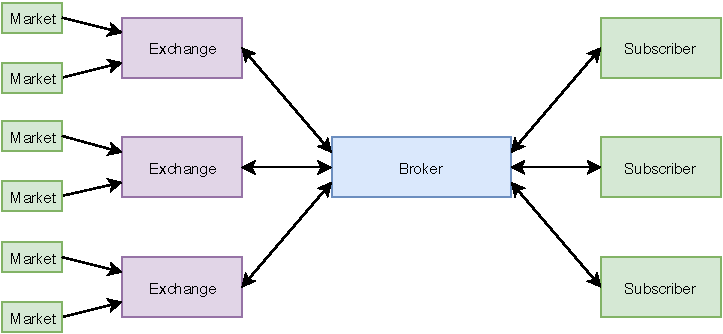
\includegraphics[width=\textwidth]{marketpull.pdf}
    \caption{blablabla}
    \label{fig:ccxt}
\end{figure}

In addition, with the reverse map we create, we can estimate the ratio of how many exchanges that has a given market. As this was one characteristics of a \ac{pd} described in \autoref{tab:pd_characteristics}. Before the master collects the \ac{ohlc} market values, we take the mean of them.

\subsubsection{CoinMarketCap}
The final slave retrieve data from \href{https://coinmarketcap.com/}{CoinMarketCap}, which is a popular cryptocurrency tracking site and contains general information regarding coins like its capitalization, circulation, and etc. We have to use CoinMarketCap private \ac{api} as they deprecated their public \ac{api}. Using their private \ac{api} is relatively intuitive, the identification is an \ac{api} key, but CoinMarketCap has defined a severe complex request system. Where a user has a load of credits, and the amount of credit one have depends on the type of subscription. In addition, a user also has a daily, weekly, and monthly request rate system, which also depends on the type of subscription on have. There are some Python modules in existence that allows one to extract data from CoinMarketCap, but they completely ignore the request system, which, when used will be problematic as we continuously will exceed the request limit and credit system, which ultimately results in a permanent ban from using their \ac{api}.

Thus, we create our own module that support throttling of requests, which adjusts to both the credit system and the number of request one can issue. We cache every request in a database because CoinMarketCap mostly provide data that rarely or slightly change. The cache also comes with an exceed factor allowing one to adjust when cached data shall be removed from the cache. There are four endpoints in CoinMarketCap, where each endpoints has a set of functions:
\begin{itemize}
    \item Cryptocurrency
    \item Exchanges
    \item Globals
    \item Tools
\end{itemize}

We use the modules requests, requests\_cache, and ratelimit. The requests module is module for making requests. Requests\_cache is monkey patch to the request module, and caches every request made by the request module. The ratelimit allows to define function descriptors that restricts the number of function calls within a time scope.

With the module we create, we fetch data from the cryptocurrency endpoints. The majority of the functions in CoinMarketCap requires a paid subscription. We are only using two free functions. The first function returns the global metrics, which contains the important value, total market capitalization. The second function lists cryptocurrencies latest market data that contains the fields circulation supply for each market, it defines the total amount of cryptocurrency worth. The reason we do not use the trading data that CoinMarketCap is because we cache every request, resulting in using stale trading data.

\section{Data Processing}
After gathered enough data, we can start process it. Each market has it own file containing data from all the sources recently described, and since they has to be processed equally, we can parallelize each operation, allowing us to speedup the data processing stage. Each file we have to process can be small in general, but combining them all together they may become quite large. Hence, we only process a fixed number of files in parallel. 

We paralellize every operation by allowing the master process to spawn new child processes. The master initialize every child process with a semaphore and queue. The first process do when they wake up is to grant access to run in a critical space, if their request gets rejected, they has to wait in queue. Once gets inside the critical area, they load the dataset using Pandas and execute the operation they are assigned to do. After they are done with their task, they signalize to the master process using a queue that they are done, and when leaving the critical section, next child process can enter it.

With data loaded into a date frame in Pandas, we index features by their column name, which makes it convinient when we do cleansing and feature engineering. 
% cleanse

The first number of operations involves cleansing the data. We cleanse by removing corrupted files, in some cases, e.g Binance have deleted markets and removed the possibility of extracting trading data from it, which results in corrupt data. We also remove the features that are not needed, e.g, in \autoref{code:bianance_tick}, the constant categorical field \texttt{symbol} are not needed when classifying \ac{pd}. The last cleansing process we do is to interpolate the data. Values involving price and quantity gets linearly interpolated like we describe in \autoref{ch:design}.

The second series of operation we do is to create new features. We calculate the percentage of change like described in \autoref{ch:design} on all the values we interpolated. Then we create new features from using the timestamp that we added along with the data when it was stored. Finally, we create a new feature that describe the imbalance of the order book.

\section{Collecting pump-and-dumps}
When collecting \acp{pd}, we use an anomaly detection algorithm that marks an interval if there was a significant increase of price and volume in that period compared to the previous periods. We do not use the anomaly detection algorithm with the data that was collected in real-time, as this data is not compliant with the algorithm. Instead, we retrieve historical \ac{ohlc} data from Binance that span over the period we gathered data.

The algorithm takes in a window (list) with a fixed number of \ac{ohlcv} values. The window is smaller than the batch of ordered \ac{ohlc} values receieve. So we create a sliding window module which is wraps round a python list. With the sliding window, it becomes is easy initialize a fixed size list, and when adding new element to the list, the last element will be removed. Just like a fixed size \ac{fifo} structure.

\autoref{binance_kline} illustrates an entry in a response from Binance that contains historical klines. With both the klines and a sliding window, we start to contionoussly add \ac{ohlcv} values that span over one hour to the window until it is full, then we iteratively calculate weather the newest added \ac{ohlc} is an anomaly compared to the other \ac{ohlc} values in the window. The fields we use from the data are \texttt{close} and \texttt{high} when calculating the price anomaly, while we only use the field \texttt{volume} when calculating the volume anomaly. The formula we use is described in \autoref{ch:design}

\begin{lstlisting}[language=json, caption={Historical kline response from Binance (Source \cite{binance_git})}, label=code:binance_kline, firstnumber=1]
[
  [
    1499040000000,      // Open time
    "0.01634790",       // Open
    "0.80000000",       // High
    "0.01575800",       // Low
    "0.01577100",       // Close
    "148976.11427815",  // Volume
    1499644799999,      // Close time
    "2434.19055334",    // Quote asset volume
    308,                // Number of trades
    "1756.87402397",    // Taker base volume
    "28.46694368",      // Taker quote volume
  ]
]
\end{lstlisting}

As we have previously mentioned, anomaly detection algorithm tends to have a high occurrences of false-positive compared to true-positive. So we filter them out by plotting finer-grained \ac{ohlc} values from the period that was flagged anomalous from each market. We can plot these \ac{ohlc} values by using the matplotlib module in Python. The chart that seems like a \ac{pd} occured we keep, otherwise we delete that anomaly.

After filtering out the \ac{pd} that seemingly looks like true positives, we can label the the features we created weather that point was collected during a \ac{pd} or not. We use the same parallize processing model, which we used during the feature engineering stage. where each process is iniated with a semaphore and queue, but also the \ac{pd} the periods where a \ac{pd} happened in the data. Then, the child process loads the dataset and idientify the interval where the \ac{pd} occured, and find the points where largest change in price percent happened. From the highest point, we label the points \ac{pd} where the change in percent was positive.

\section{Deep Learning}
After we have generated labeled datasets, we normalize each of them using the min-max method described in \autoref{ch:design}. To find the smallest and biggest value of each feature require us to process trough all of the datasets in order to find the largest sand smallest value in each feature. Then, when we have these value we have to process normalize every row. We use one functions from the scikit-learn package when normalizing the data.

In our implementation, we use the method undersampling when generating a balanced dataset. So, first we have to collect all the positive samples. Then we simply choose random negative sequences from the dataset until the number of negative and positive samples are equal.

we use the deep learning library Keras for our model, the first layer contains active \ac{lstm} cells, and the second layer contains a single perceptron.

Before training a \acp{lstm} network, we need to resphape our input data, which is a matrix, a 2D shape, into 3D shape. A sample now, is a matrix containing batch of row-vectors within a time lag. Then the third dimensions is simply batch of these new samples. After shaping our data, we can finallyu train our model.


% Measurement results / analysis / discussion:
% whatever you have done, you must comment it, compare it to other systems, evaluate it
% usually, adequate graphs help to show the benefits of your approach
% caution: each result/graph must be discussed! what’s the reason for this peak or why have you ovserved this effect

\chapter{Evaluation}\label{ch:evaluation}\glsresetall
\section{Experimental Setup}\label{sec:experimental_setup}
To evaluate \project, we investigate its model prediction capabilities, and we did so by retrieving real-time data from $138$ different markets throughout $33$ days. The pairing coin of each market was Bitcoin. The interval between each data point was $5$ seconds, resulting in approximately $\numprint{570 000}$ samples per market. Over these days, we collected in total \SI{47}{\giga\byte} of data. The sources that we use to fetch data from was those we presented in the \autoref{ch:implementation}, namely, Binance, CoinMarketCap, and aggregated data from multiple sources. 

\autoref{tab:feature_table} contains details regarding every feature that were fetched. The operation fields describe how we decided to process a specific feature. The data were cleaned by removing features that we believe was unproductive in the detection of \ac{pd}, these were tagged as \emph{Remove}. The field that contains \emph{PoC}, was first interpolated and then calculated the percentage of change, and the time lag we chose was $10$ minutes because the time from where a \ac{pd} start, to where it peak is $10$ minutes, like described in \autoref{ch:background}. The field \emph{Imbalance} and \emph{Time} are the order book imbalance and how close the timestamp is on the hour.

\begin{table}
    \centering
    \begin{tabular}{|l|l|l|l|}
    \hline
            Source          & Symbol        & Feature Description           & Operation \\\hline
            Local           & $dt$          & Local timestamp               & Time      \\
            Binance         & $e$           & Event type                    & Removed   \\
            Binance         & $E$           & Event time                    & Removed   \\
            Binance         & $s$           & Symbol                        & Removed   \\
            Binance         & $P$           & Price change percent          & None      \\
            Binance         & $p$           & Price change                  & PoC       \\
            Binance         & $w$           & Weighted average price        & PoC       \\
            Binance         & $x$           & First trade(F)-1 price        & PoC       \\
            Binance         & $c$           & Last price                    & PoC       \\
            Binance         & $Q$           & Last quantity                 & PoC       \\
            Binance         & $b$           & Best bid price                & PoC       \\
            Binance         & $B$           & Best bid quantity             & PoC       \\
            Binance         & $a$           & Best ask price                & PoC       \\
            Binance         & $A$           & Best ask quantity             & PoC       \\
            Binance         & $o$           & Open price                    & PoC       \\
            Binance         & $h$           & High Price                    & PoC       \\
            Binance         & $l$           & Low Price                     & PoC       \\
            Binance         & $v$           & Base asset volume             & PoC       \\
            Binance         & $q$           & Quote asset volume            & PoC       \\
            Binance         & $O$           & Statistics open time          & Removed   \\
            Binance         & $C$           & Statistics close time         & Removed   \\
            Binance         & $F$           & First trade ID                & Removed   \\
            Binance         & $L$           & Last trade ID                 & Removed   \\
            Binance         & $n$           & Total number of trades        & PoC       \\
            Binance         & $ap\_[0-4]$   & $5$x depth - asks price       & PoC       \\
            Binance         & $av\_[0-4]$   & $5$x depth - asks volume      & PoC       \\
            Binance         & $bp\_[0-4]$   & $5$x depth - bids price       & PoC       \\
            Binance         & $av\_[0-4]$   & $5$x depth - asks volume      & PoC       \\
            Binance         & $dep$         & Depth imbalance               & Imbalance \\
            ccxt            & $oc$          & Aggregated open price         & PoC       \\
            ccxt            & $hc$          & Aggregated high price         & PoC       \\
            ccxt            & $lc$          & Aggregated low price          & PoC       \\
            ccxt            & $cc$          & Aggregated close price        & PoC       \\
            ccxt            & $ic$          & Exchange to market rate       & None      \\
            CoinMarketCap   & $cap$         & Capitalization rate           & None      \\
    \hline
    \end{tabular}
    \caption[Features used]{This is all the features we fetched and used to train our model.}
    \label{tab:feature_table}
\end{table}


We used the anomaly detection algorithm which we have previously described to pinpoint \ac{pd} intervals. We fetched \ac{ohlc} values that span over the period we collected data, and these \ac{ohlc} values had an interval of $1$ hour. The threshold parameters we chose for the algorithm is a price increase of $1.10$ and a volume of increase threshold of $3.00$, and the time lag we chose was $6$ hour. By using this algorithm we were able to identify in total $280$ anomalies. Of these anomalies we manually removed $80$, which we believe was false. \autoref{fig:label_true} shows three \acp{pd} charts we believe was true, while \autoref{fig:label_false} shows three \ac{pd} charts we believe was false.

\begin{figure}
    \centering
    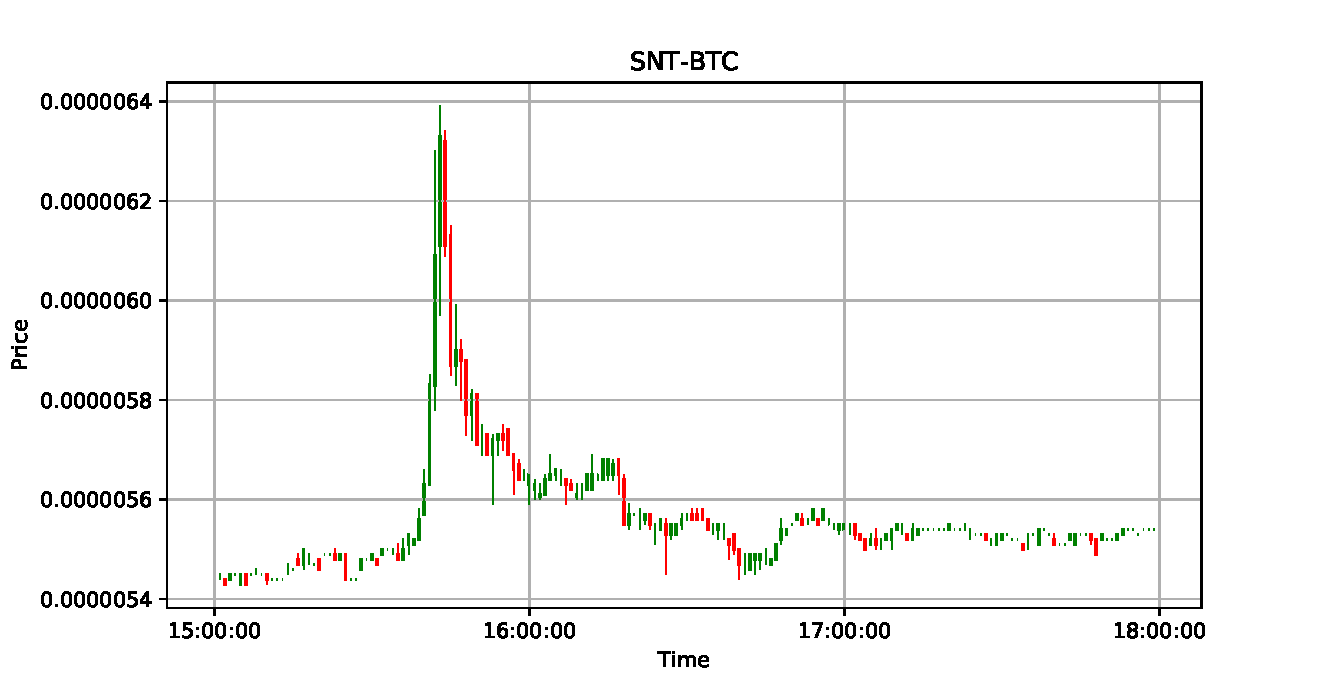
\includegraphics[width=\textwidth]{true_1.pdf}
    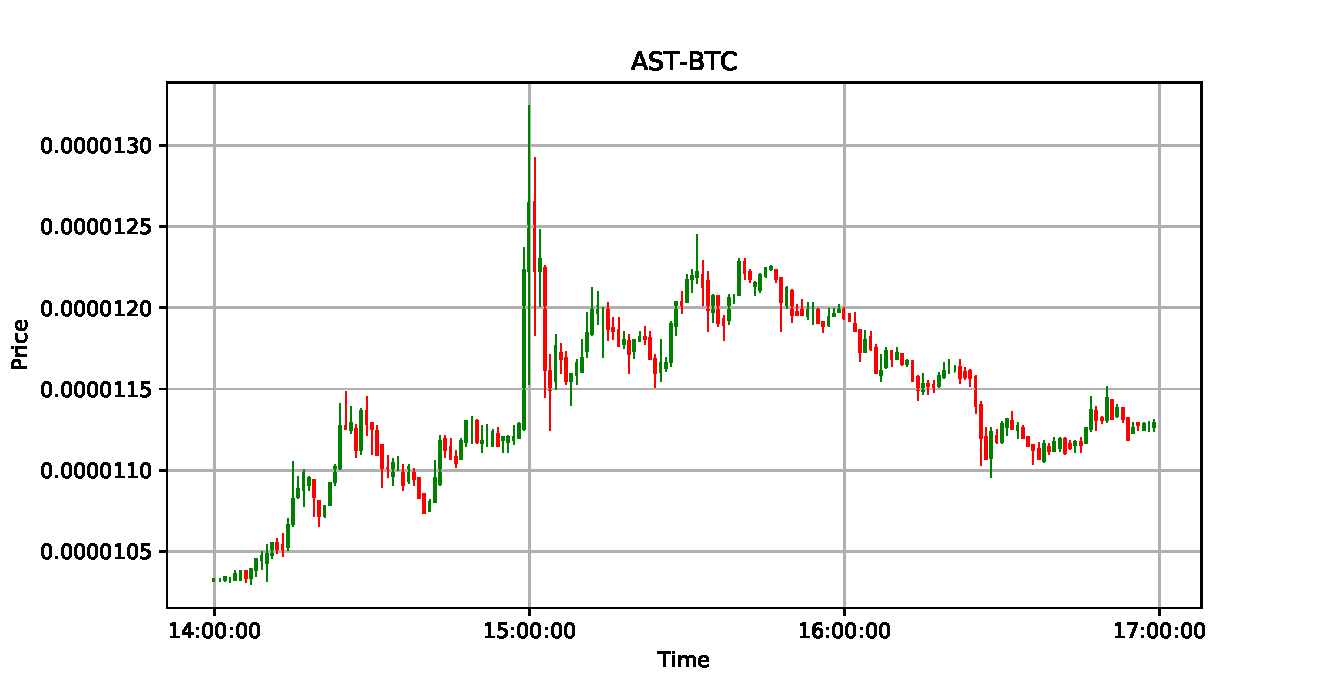
\includegraphics[width=\textwidth]{true_2.pdf}
    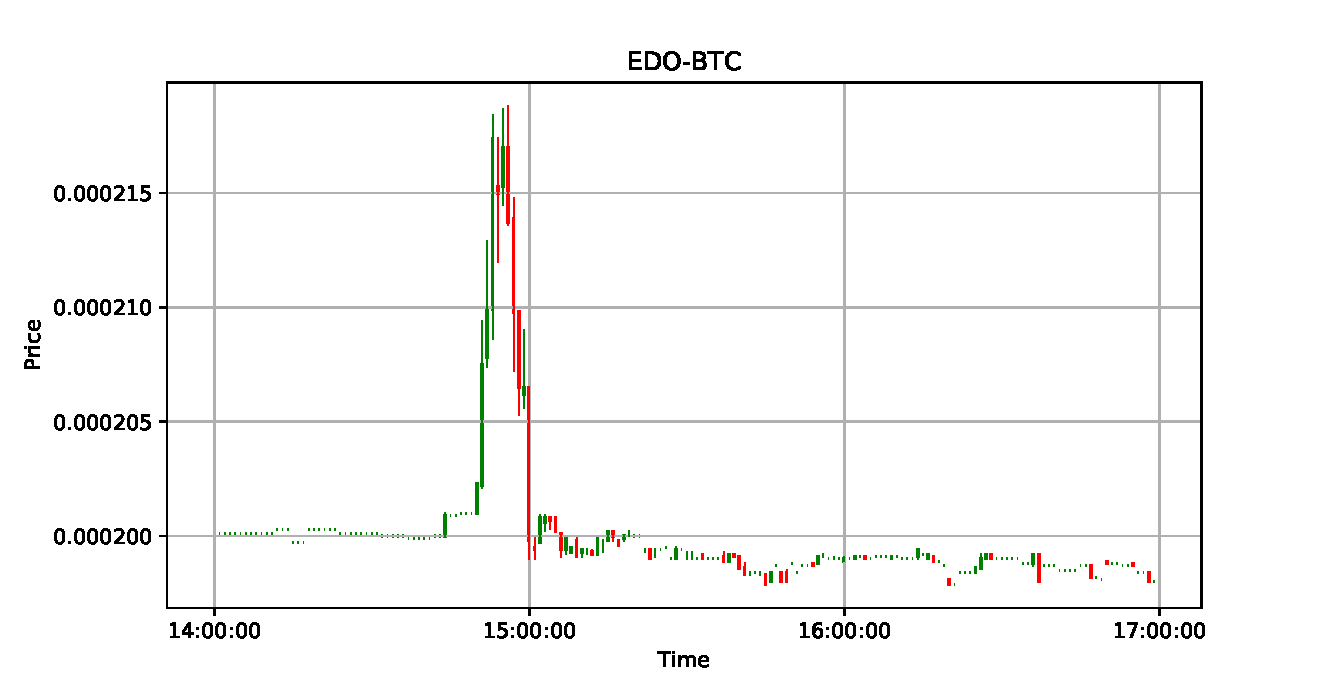
\includegraphics[width=\textwidth]{true_3.pdf}
    \caption{Anomalies that seems like a \ac{pd}}
    \label{fig:label_true}
\end{figure}

\begin{figure}
    \centering
    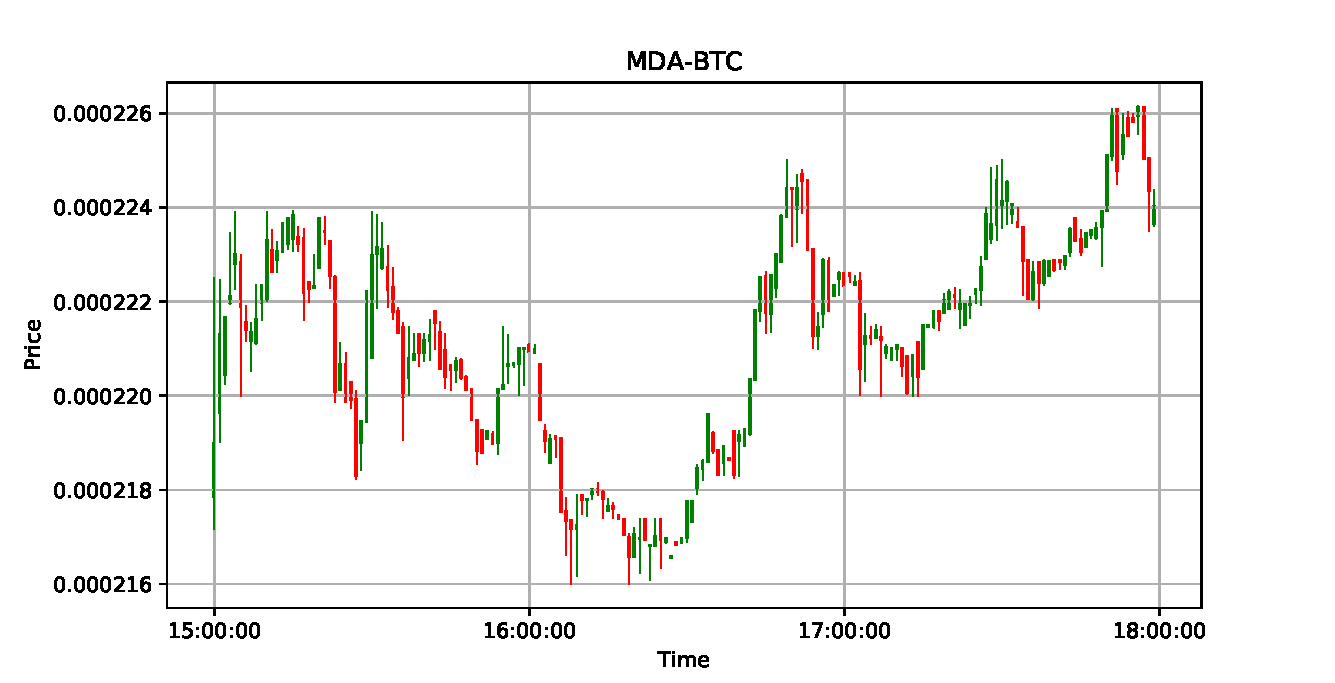
\includegraphics[width=\textwidth]{false_1.pdf}
    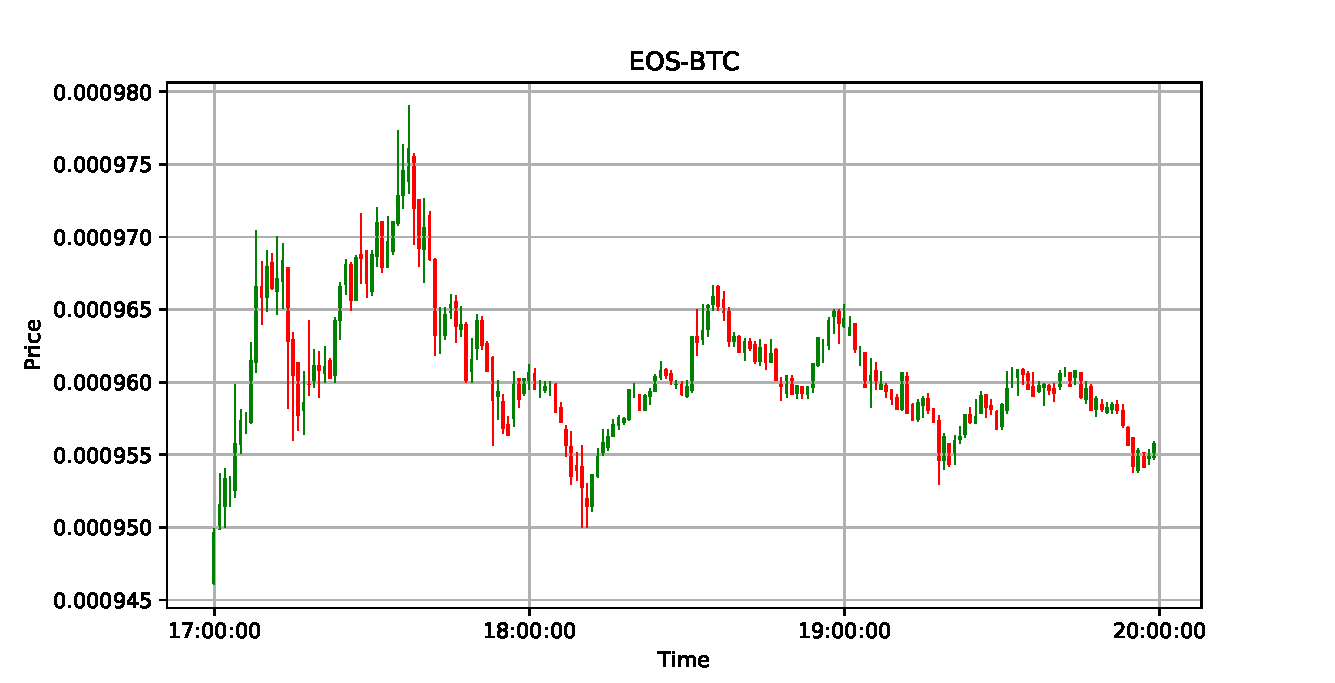
\includegraphics[width=\textwidth]{false_2.pdf}
    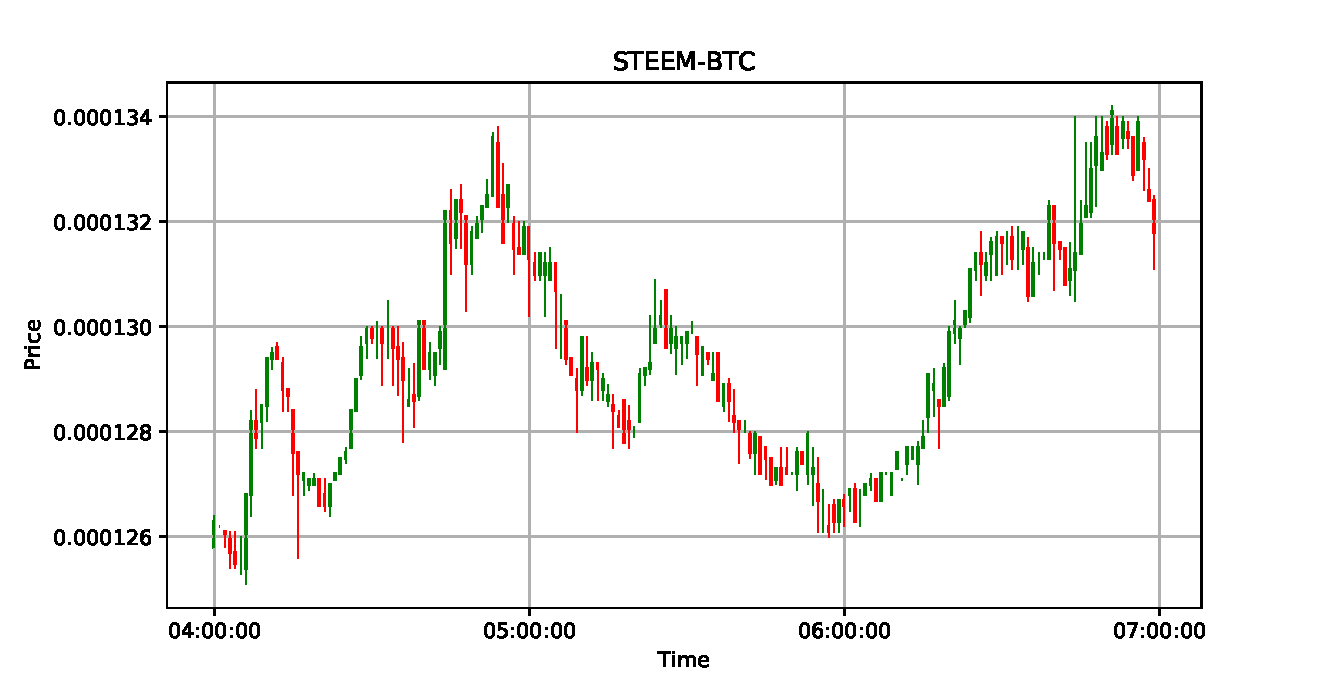
\includegraphics[width=\textwidth]{false_3.pdf}
    \caption{Anomalies that not seems like a \ac{pd}}
    \label{fig:label_false}
\end{figure}

To create a dataset, we used the anomalies to label all the processed, collected data. The generated dataset was then normalized by using the min-max normalization method. We split the dataset into a training set and a test set. The training set was consist of $75\%$ of the dataset, resulting in data from approximately $104$ markets, while the test set contains the remaining $25\%$ of the markets, resulting in $33$ markets. The training dataset was undersampled in order to create a balanced dataset.

The network we used was a \ac{lstm} network, where its hidden layer contains a single layer with $50$ \ac{lstm} cells, where each cell had a "short memory" of $10$ points, which results in $50$ seconds of memory considering that interval between each sample is $5$ seconds. We also added dropout to prevent over-fitting as \ac{lstm} cells tend to overfit their training data often~\cite{overfit}. The output layer contained a single perceptron. The optimizer we used was \emph{adam}, which is an extension to stochastic gradient descent~\cite{kingma2014adam}, the optimizer has shown that the model's weights will converge faster that results in greater performance rapidly~\cite{adam}. The network was trained in over $5000$ epochs with the training dataset, where the batch size was $10$. To define the performance of the network, we classified all the samples in the test dataset and rounded the probabilistic prediction to either $0$ (\ac{pd}) or $1$ (not \ac{pd}). 

The computer we used to train our model with had the following specifications:
\begin{itemize}
    \item CPU - Intel Xeon E5-1620 \SI{3.9}{\giga\hertz}
    \item RAM - \SI{64}{\gibi\byte} DDR3 
    \item GPU - Nvidia GeForce GTX 770
\end{itemize}
\newpage

\section{Results}
The first metric we use is a confusion matrix, which is structured like \autoref{tab:confmat}. A confusion matrix shows the number of correct and incorrect classified samples, and help define further scores. True positive $tp$ are samples that are correctly classified as \ac{pd}, while true negative, $tn$, is samples that are correctly classified as not \ac{pd}. $fp$ are samples that are incorrect classified as \ac{pd}, and false negatives, $fn$, are samples that are \ac{pd}, but classified as not \ac{pd}. $p$ and $n$ are the true total numbers of samples in each class, while $p'$ and $n'$ are the total numbers of predicted samples in each class. Finally, $N$ is the total number of samples.

\begin{table}
    \centering
    \begin{tabular}{|c|c|c|c|}\hline
                &   \multicolumn{3}{c|}{Predicted class}\\\hline
    True class  &  Positive             & Negative              & Total \\\hline
    Positive    & $tp$: true positive   & $fn$: false negative  & $p$   \\
    Negative    & $fp$: false positive  & $tn$: true negative   & $n$   \\\hline
    Total       & $p'$                  & $n'$                  & $N$   \\\hline
    \end{tabular}
    \caption{Confusion matrix}
    \label{tab:confmat}
\end{table}
\begin{table}
        \centering
        \begin{tabularx}{\textwidth}{ |R|R|R|R| }\hline
                    &   \multicolumn{3}{c|}{Predicted class}\\\hline
        True class  & Positive              & Negative              & Total                 \\\hline
        Positive    & $\numprint{7910}$     & $\numprint{911}$      & $\numprint{8821}$     \\
        Negative    & $\numprint{388795}$   & $\numprint{17933021}$ & $\numprint{18321816}$ \\\hline
        Total       & $\numprint{396705}$   & $\numprint{17933932}$ & $\numprint{18330637}$ \\\hline
        \end{tabularx}
        \caption{\project's confusion matrix}
        \label{tab:model_performance}
\end{table}

As we can see from \autoref{tab:model_performance}, the test dataset, as well as the training dataset is hugely imbalanced. Only $\numprint{8821}$ samples are \ac{pd}, while $\numprint{18321816}$ is not a \ac{pd}. Over one of every $\numprint{2000}$ sample is a \ac{pd}!

\begin{table}
    \centering
    \begin{tabular}{|c|c|r|}\hline
    Name        & Formula       &   Result      \\\hline
    error       & $(fp+fn)/N$   &   $0.0217$    \\
    accuracy    & $(tp+tn)/N$   &   $0.9782$    \\\hline
    tp-rate     & $tp/p$        &   $0.8967$    \\
    fp-rate     & $fp/n$        &   $0.0212$    \\\hline
    sensitivity & $tp/p$        &   $0.8967$    \\
    specificity & $tn/n$        &   $0.9787$    \\\hline
    recall      & $tp/p$        &   $0.8967$    \\
    precision   & $tp/p'$       &   $0.0199$    \\\hline
    \end{tabular}
    \caption{Performance measure}
    \label{tab:performance}
\end{table}

From \autoref{tab:performance}, we see various metrics that we can use when defining the capabilities of the \ac{lstm} network, the metrics \emph{accuracy} and \emph{error}, are measures that are opposite of each other. The accuracy is the percentage of how many samples we classified correct. The error, says how many samples we misclassified. 

\begin{figure}[ht]
    \centering
    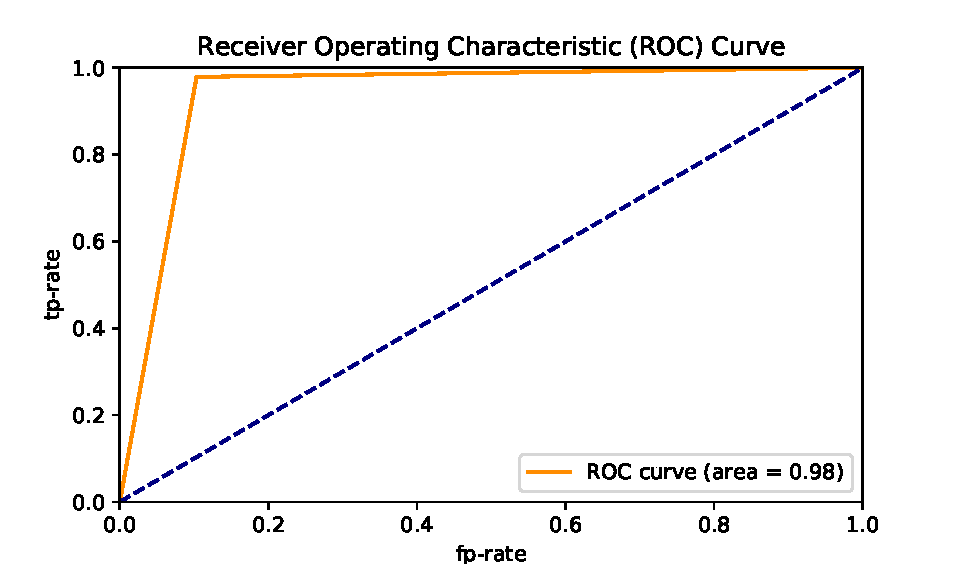
\includegraphics[width=\textwidth]{results/roc.pdf}
    \caption{Roc Curve}
    \label{fig:roc}
\end{figure} 

The tp-rate is percentage of how often we correctly classify \ac{pd} samples. So given a \ac{pd} sample, there an $89.67\%$ chance of classifying it correctly. The fp-rate is similar in terms of, given a negative sample. Then there is a $2.12\%$ change of classifying it at as a \acp{pd}. These measures can also be visualized through \ac{roc} curve illustrated in \autoref{fig:roc}. It gives us a visual perspective of the performance of the model. Ideally, a classifier has a tp-rate of $1$ and an fp-rate of $0$, and a classifier is better the more its \ac{roc} curve gets closer to the upper-left corner. On the diagonal, we make as many true decisions as false ones, and this is the worst case~\cite[p.~563]{alpaydin2014introduction}. Our \ac{roc} curve also shows that our model has accurate predictable capabilities. The \ac{auc} score represents the probability that a randomly chosen positive example is correctly classified ranked with greater suspicion than a randomly chosen negative example~\cite{bradley1997use}.
The \emph{sensitivity} and \emph{specificity} balance the classes, they tells us, given a negative or positive samples, what is the percentage of classifying it correctly. The sensitivity, is the percentage of given a positive sample, the percentage of classifying it correctly, is $89.67\%$. The specificity, is the opposite, given a negative sample, the percentage of classifying it correctly is $97.87\%$. 

Clearly, the metrics we presented now shows that the model has good predictable capabilities. However, the metrics that reveal the flaws of the model, are the measures \emph{recall} and \emph{precision}. Recall are exactly like the tp-rate and sensitivity, it is the percentage of, given a \ac{pd} sample, then there is $89.67\%$ chance of classifying it correctly. \emph{precision} on the other hand, is, if classifying a sample as a \ac{pd}, then, what is the percentage that the sample truly is a \ac{pd}. In our case, a disappointing $1.99\%$. so whenever our model predicts a \ac{pd}, then there is only a $1.99\%$ that it is correct, and this results in plenty of false alarms.

\begin{align}\label{eq:f_score}
    F_\beta &= (1+\beta^2) \cdot \frac{\text{precision} \cdot \text{recall}}{(\beta^2\cdot\text{precision}) + \text{recall}},\quad
    \begin{cases} 
    F_{0.5} &= 0.0247\\ 
    F_1     &= 0.0389\\ 
    F_2     &= 0.0912\\ 
    \end{cases}
\end{align}

A frequently used score that relies on recall and precision is the \emph{f-score}. The f-score formula is showed in \autoref{fig:f_score}, and an ideal f-score is $1$, and the worst is $0$. This measure is flexible in terms that we can weigh both recall and precision differently by adjusting the parameter $\gamma$. Where the closer $\gamma$ is to $0$, the more we weigh precision, when $\gamma$ is $1$ we wight them equally, and finally when $\gamma$ is over $1$, we weigh recall most. As we see, when weighing precision most, by giving  $\gamma=0.5$, the score only yield $0.0247$. When equally weighing them, by giving $\gamma=1$, the score increase slightly. Finally, when weighting recall most, the score is $0.0912$, which is better than the other.

The following results shows the confusion matrix of each classified market.

\begin{table}[H]
        \centering
        \begin{tabularx}{\textwidth}{ |R|R||R|R||R|R| }
                \multicolumn{2}{c}{WABI-BTC} & \multicolumn{2}{c}{MITH-BTC} & \multicolumn{2}{c}{ETH-BTC} \\\hline
                $\numprint{376}$\cellcolor{green!91} & $\numprint{36}$\cellcolor{red!9} & $\numprint{0}$\cellcolor{green!0} & $\numprint{2}$\cellcolor{red!100} & $\numprint{0}$\cellcolor{green!100} & $\numprint{0}$\cellcolor{red!0} \\
                $\numprint{23440}$\cellcolor{red!5} & $\numprint{531622}$\cellcolor{green!95} & $\numprint{26798}$\cellcolor{red!5} & $\numprint{528675}$\cellcolor{green!95} & $\numprint{0}$\cellcolor{red!0} & $\numprint{555474}$\cellcolor{green!100} \\
                \hline
                \addlinespace[.2cm]

                \multicolumn{2}{c}{XRP-BTC} & \multicolumn{2}{c}{BTT-BTC} & \multicolumn{2}{c}{OST-BTC} \\\hline               
                $\numprint{0}$\cellcolor{green!100} & $\numprint{0}$\cellcolor{red!0} & $\numprint{0}$\cellcolor{green!100} & $\numprint{0}$\cellcolor{red!0} & $\numprint{488}$\cellcolor{green!90} & $\numprint{53}$\cellcolor{red!10} \\
                $\numprint{0}$\cellcolor{red!0} & $\numprint{555474}$\cellcolor{green!100} & $\numprint{3400}$\cellcolor{red!1} & $\numprint{552074}$\cellcolor{green!99} & $\numprint{8705}$\cellcolor{red!2} & $\numprint{546228}$\cellcolor{green!98} \\
                \hline
                \addlinespace[.2cm]

                \multicolumn{2}{c}{CDT-BTC} & \multicolumn{2}{c}{GNT-BTC} & \multicolumn{2}{c}{TRX-BTC} \\\hline               
                $\numprint{407}$\cellcolor{green!88} & $\numprint{51}$\cellcolor{red!12} & $\numprint{375}$\cellcolor{green!78} & $\numprint{105}$\cellcolor{red!22} & $\numprint{0}$\cellcolor{green!100} & $\numprint{0}$\cellcolor{red!0} \\
                $\numprint{18303}$\cellcolor{red!4} & $\numprint{536713}$\cellcolor{green!96} & $\numprint{20994}$\cellcolor{red!4} & $\numprint{534000}$\cellcolor{green!96} & $\numprint{289}$\cellcolor{red!1} & $\numprint{555185}$\cellcolor{green!99} \\
                \hline
                \addlinespace[.2cm]

                \multicolumn{2}{c}{MTH-BTC} & \multicolumn{2}{c}{DLT-BTC} & \multicolumn{2}{c}{SC-BTC} \\\hline                
                $\numprint{487}$\cellcolor{green!97} & $\numprint{16}$\cellcolor{red!3} & $\numprint{584}$\cellcolor{green!87} & $\numprint{85}$\cellcolor{red!13} & $\numprint{0}$\cellcolor{green!100} & $\numprint{0}$\cellcolor{red!0} \\
                $\numprint{12032}$\cellcolor{red!3} & $\numprint{542939}$\cellcolor{green!97} & $\numprint{19223}$\cellcolor{red!3} & $\numprint{535580}$\cellcolor{green!97} & $\numprint{7234}$\cellcolor{red!2} & $\numprint{548240}$\cellcolor{green!98} \\
                \hline
                \addlinespace[.2cm]

                \multicolumn{2}{c}{SNT-BTC} & \multicolumn{2}{c}{XEM-BTC} & \multicolumn{2}{c}{VIB-BTC} \\\hline                
                $\numprint{323}$\cellcolor{green!88} & $\numprint{40}$\cellcolor{red!12} & $\numprint{0}$\cellcolor{green!100} & $\numprint{0}$\cellcolor{red!0} & $\numprint{674}$\cellcolor{green!99} & $\numprint{7}$\cellcolor{red!1} \\
                $\numprint{8138}$\cellcolor{red!2} & $\numprint{546973}$\cellcolor{green!99} & $\numprint{914}$\cellcolor{red!1} & $\numprint{554559}$\cellcolor{green!99} & $\numprint{22358}$\cellcolor{red!5} & $\numprint{532435}$\cellcolor{green!95} \\
                \hline
                \addlinespace[.2cm]

                \multicolumn{2}{c}{MTL-BTC} & \multicolumn{2}{c}{HC-BTC} & \multicolumn{2}{c}{STORM-BTC} \\\hline             
                $\numprint{477}$\cellcolor{green!93} & $\numprint{36}$\cellcolor{red!7} & $\numprint{251}$\cellcolor{green!57} & $\numprint{188}$\cellcolor{red!43} & $\numprint{0}$\cellcolor{green!100} & $\numprint{0}$\cellcolor{red!0} \\
                $\numprint{29687}$\cellcolor{red!6} & $\numprint{525274}$\cellcolor{green!94} & $\numprint{5213}$\cellcolor{red!1} & $\numprint{549822}$\cellcolor{green!99} & $\numprint{14995}$\cellcolor{red!3} & $\numprint{540479}$\cellcolor{green!97} \\
                \hline
                \addlinespace[.2cm]

                \multicolumn{2}{c}{INS-BTC} & \multicolumn{2}{c}{LUN-BTC} & \multicolumn{2}{c}{NXS-BTC} \\\hline               
                $\numprint{0}$\cellcolor{green!0} & $\numprint{1}$\cellcolor{red!100} & $\numprint{792}$\cellcolor{green!93} & $\numprint{57}$\cellcolor{red!7} & $\numprint{0}$\cellcolor{green!100} & $\numprint{0}$\cellcolor{red!0} \\
                $\numprint{7032}$\cellcolor{red!2} & $\numprint{548439}$\cellcolor{green!98} & $\numprint{12443}$\cellcolor{red!3} & $\numprint{542182}$\cellcolor{green!97} & $\numprint{6554}$\cellcolor{red!1} & $\numprint{548920}$\cellcolor{green!99} \\
                \hline
                \addlinespace[.2cm]

                \multicolumn{2}{c}{TNB-BTC} & \multicolumn{2}{c}{NPXS-BTC} & \multicolumn{2}{c}{ZRX-BTC} \\\hline               
                $\numprint{441}$\cellcolor{green!99} & $\numprint{3}$\cellcolor{red!1} & $\numprint{0}$\cellcolor{green!100} & $\numprint{0}$\cellcolor{red!0} & $\numprint{0}$\cellcolor{green!100} & $\numprint{0}$\cellcolor{red!0} \\
                $\numprint{47144}$\cellcolor{red!9} & $\numprint{507886}$\cellcolor{green!91} & $\numprint{3381}$\cellcolor{red!1} & $\numprint{552093}$\cellcolor{green!99} & $\numprint{10138}$\cellcolor{red!2} & $\numprint{545336}$\cellcolor{green!98} \\
                \hline
                \addlinespace[.2cm]

                \multicolumn{2}{c}{VET-BTC} & \multicolumn{2}{c}{RCN-BTC} & \multicolumn{2}{c}{ETC-BTC} \\\hline                
                $\numprint{0}$\cellcolor{green!100} & $\numprint{0}$\cellcolor{red!0} & $\numprint{487}$\cellcolor{green!95} & $\numprint{26}$\cellcolor{red!5} & $\numprint{160}$\cellcolor{green!84} & $\numprint{30}$\cellcolor{red!16} \\
                $\numprint{1321}$\cellcolor{red!2} & $\numprint{554153}$\cellcolor{green!98} & $\numprint{10697}$\cellcolor{red!2} & $\numprint{544264}$\cellcolor{green!98} & $\numprint{2890}$\cellcolor{red!1} & $\numprint{552394}$\cellcolor{green!99} \\
                \hline
                \addlinespace[.2cm]

                \multicolumn{2}{c}{SNM-BTC} & \multicolumn{2}{c}{SKY-BTC} & \multicolumn{2}{c}{LOOM-BTC} \\\hline              
                $\numprint{1209}$\cellcolor{green!95} & $\numprint{55}$\cellcolor{red!5} & $\numprint{141}$\cellcolor{green!76} & $\numprint{44}$\cellcolor{red!24} & $\numprint{0}$\cellcolor{green!100} & $\numprint{0}$\cellcolor{red!0} \\
                $\numprint{21950}$\cellcolor{red!4} & $\numprint{532260}$\cellcolor{green!96} & $\numprint{14423}$\cellcolor{red!2} & $\numprint{540866}$\cellcolor{green!98} & $\numprint{1485}$\cellcolor{red!1} & $\numprint{553989}$\cellcolor{green!99} \\
                \hline
                \addlinespace[.2cm]

                \multicolumn{2}{c}{CVC-BTC} & \multicolumn{2}{c}{PHX-BTC} & \multicolumn{2}{c}{PPT-BTC} \\\hline               
                $\numprint{238}$\cellcolor{green!76} & $\numprint{74}$\cellcolor{red!24} & $\numprint{0}$\cellcolor{green!0} & $\numprint{1}$\cellcolor{red!100} & $\numprint{0}$\cellcolor{green!0} & $\numprint{1}$\cellcolor{red!100} \\
                $\numprint{8393}$\cellcolor{red!1} & $\numprint{546769}$\cellcolor{green!99} & $\numprint{13211}$\cellcolor{red!2} & $\numprint{542262}$\cellcolor{green!98} & $\numprint{6010}$\cellcolor{red!1} & $\numprint{549463}$\cellcolor{green!99} \\
                \hline
        \end{tabularx}
        \caption[\project's confusion matrices of tested markets]{confusion matrices of the $33$ tested markets.}
        \label{tab:results}
\end{table}

\newpage
\section{Discussion}
To interpret the results reasonable, we need to define the potential consequences of a misclassification. So, to push it to the extreme, assume our real job was to classify whether a patient has cancer using machine learning. The model we use to predict cancer has already be trained and does have accurate predictions, but like many other models, it is not entirely flawless, and occasionally it will make an incorrect prognosis of cancer. At some point, the model makes a wrong decision, and it predicts that a patient has cancer, while the patient is actually cancer free. The consequences might be that the patient is starting a treatment, it can also have other side effects that impact her or him in a somatic and psychological way, but the patient will at least live. If we turn the table, and the model predicts that a patient does not have cancer, while the patient truly has. Then, in short amount of time, the patient will die of cancer, which is an unforgivable fault made by us. This example only clarifies the potential harm of misclassifications, and it is not like that any will die from misclassifying \acp{pd}, hopefully.

So to apply the consequence of misclassifications in the detection of \acp{pd}. Assume that, an exchange uses our model to detect \acp{pd} in order to ban users that participate in them. As we have seen, our model is not perfect, it makes wrong decisions occasionally, and just like Murphy's law, everything that can happen will happen. At some point, our model makes a wrong decision and predicts a \ac{pd} and the exchange ban a set of investors from using their platform. Banning investors on false terms, will undermine the exchange's credibility, and have various additional consequences for them. On the other hand, missing \acp{pd} are not harmful. Despite that some investors avoid getting banned, but if the investors ever try again, they might not be so lucky.

As we saw from our results, all the metrics except f-score and precision performs excellent and excels other models that detect \acp{pd}. The f-score and precision is a fatal flaw of our model, and as the model currently is, deploying it now will be remarkably hard as there would be too many false alarms. However, there are ways to adjust the precision, but at a particular cost. Improving it will with a high likelihood cost us our current tp-rate and make that worse, but due to the nature of the metrics, increasing precision will also increase some other measures. As changing the precision means, either increase the true positives or decrease false positives.

Increasing true positives in our case can make precision worse, as we must try to make the model fit to additional positives samples simultaneously as there are over $\numprint{2000}$ more negative samples. So, our angle should be to decrease the false positives, in order to increase precision, but that may result in a decrease of true positives. 

To adjust the false positives, we can be more strict in terms when classifying, as mentioned in end of \autoref{sec:experimental_setup}, we rounded each prediction, probabilities over $0.5$ is classified as negative, while probabilities under $0.5$ is classified as positive. If the prediction is precisely on the $0.5$ threshold, then the model can not separate it, but this case is scarce, and a case we often entirely ignore. However, the point is that we can adjust this $0.5$ threshold in terms of strict we want to be. By lowering this threshold, we can be more strict, we can be more "sure" of whether it genuinely is a \ac{pd} or not. This method also very flexible as the threshold is simple to adjust and do not require us to train our network again.

Other methods to adjust false positives is, with a purpose, to train a network with an imbalanced dataset that inclines the negative class. However, this method is not preferred as it requires to retrain the model over and over again to evaluate it. This method was also our first trial, which, when evaluating it resulted in an astonishing $99.99\%$. However, there was only one problem, it could not recognize any \acp{pd}, it classified all samples as negative.

We also tried to adjust the loss cost of each the classes during training, such that it favored positive over negative. So when making a wrong decision of a \ac{pd}, the model's weight will adjust more then it would when making a wrong decision on the other way around. Ultimately, this method was error-prone and incredibly hard to control as we had to guess how much the weights should change.

Ultimately, before using \project, one should weigh the various consequences of a misclassification and adjust the decision threshold accordingly. 
% Conclusion
% summarize again what your paper did, but now emphasize more the results, and comparisons
% write conclusions that can be drawn from the results found and the discussion presented in the paper
% future work (be very brief, explain what, but not much how)

\chapter{Concluding Remarks}\label{ch:conclusion}\glsresetall

\section{Future Work}

% Bibliography and appendix
\printbibliography[heading=bibintoc,title=Bibliography]
\backmatter

\end{document}